\documentclass[12pt, a4paper, onecolumn, oneside, final]{report}

\usepackage{csquotes}
\special{papersize=210mm,297mm}
\usepackage[top=3cm,bottom=2.5cm,left=4cm,right=2.5cm]{geometry}
\usepackage{mathptmx}
\usepackage[bahasa]{babel}
\usepackage[backend=biber,style=authoryear]{biblatex}
\usepackage[utf8]{inputenc}
\usepackage{graphicx}
\usepackage{titling}
\usepackage{blindtext}
\usepackage{sectsty}
\usepackage{chngcntr}
\usepackage{etoolbox}
\usepackage{hyperref}
\usepackage{titlesec}
\usepackage{parskip}
\usepackage{tabulary}
\usepackage{longtable}
\usepackage[titles]{tocloft}

\hypersetup{colorlinks=false, pdfborder={0 0 0},}

\renewcommand{\baselinestretch}{1.5}

\chapterfont{\centering \Large}
\titleformat{\chapter}[display]
    {\Large\centering\bfseries}
    {\chaptertitlename\ \thechapter}{0pt}
        {\Large\bfseries\uppercase}

\setcounter{secnumdepth}{3}

\counterwithin{figure}{section}
\counterwithin{table}{section}

\renewcommand*{\nameyeardelim}{\addcomma\space}
\addbibresource{references.bib}

\DeclareQuoteStyle{bahasa}
    {\textquotedblleft}
    {\textquotedblright}
    [0.05em]
    {\textquotedblleft}
    {\textquotedblright}

\DefineBibliographyStrings{english}{
    and = {\&}
}

\setlength{\cftfignumwidth}{4em}

\begin{document}

    \title{Pengembangan Sistem Auto Grading Menggunakan PC Pengguna Sebagai Worker}
    \date{\today}
    \author{
        JAUHAR ARIFIN \\
        NIM: 13515049
    }

    \pagenumbering{roman}
    \setcounter{page}{0}

    \clearpage
\pagestyle{empty}

\begin{center}
\smallskip
    \Large \bfseries \MakeUppercase{\thetitle}
    \vfill
    \Large Laporan Tugas Akhir
    \vfill
    \large Disusun sebagai syarat kelulusan tingkat sarjana
    \vfill
    \large Oleh
    \Large \theauthor
    \vfill
    \begin{figure}[h]
        \centering
      	
\includegraphics[width=0.15\textwidth]{images/itb-logo}
    \end{figure}
    \vfill
    \large
    \uppercase{
        Program Studi Teknik Informatika \\
        Sekolah Teknik Elektro dan Informatika \\
        Institut Teknologi Bandung
    }

    \thedate
\end{center}
\clearpage


    \pagenumbering{roman}
    \setcounter{page}{0}
    
    \clearpage
\pagestyle{empty}

\begin{center}
\smallskip
    \Large \bfseries \MakeUppercase{\thetitle}
    \vfill
    \Large Laporan Tugas Akhir
    \vfill
    \large Oleh
    \Large \theauthor \\
    \large Program Studi Teknik Informatika \\ Sekolah Teknik Elektro dan Informatika \\ Institut Teknologi Bandung
    \vfill
    \normalsize \normalfont
    \vfill
    Bandung, 26 Desember 2018 \\
    Mengetahui, \\
    Pembimbing,
    \vfill
    \vfill
    \vfill
    Riza Satria Perdana, ST., MT. \\
    NIP. 197006091995121002
\end{center}
\clearpage


    \pagestyle{plain}
    \titleformat*{\section}{\centering\bfseries\Large\MakeUpperCase}

    \tableofcontents
    \addcontentsline{toc}{chapter}{\contentsname}\
    \listoffigures
    \addcontentsline{toc}{chapter}{\listfigurename}\
    \listoftables
    \addcontentsline{toc}{chapter}{\listtablename}
    \clearpage

    \titleformat*{\section}{\bfseries\Large}
    \pagenumbering{arabic}
    \setcounter{page}{1}
    \renewcommand{\chaptername}{BAB}
    \renewcommand{\thechapter}{\Roman{chapter}}
    
    \chapter{Pendahuluan}

\section{Latar Belakang}

\par \textit{Competitive programming} merupakan salah satu cabang lomba yang cukup populer di bidang \textit{computer science}. Pada kompetisi \textit{competitive programming}, peserta diminta menyelesaikan persoalan terkait \textit{computer science} yang diberikan oleh juri secara benar dan dalam waktu yang singkat. Beberapa instansi dan organisasi seringkali mengadakan kompetisi ini secara rutin. Perusahaan teknologi besar seperti Google dan Facebook pun seringkali mengadakan kompetisi \textit{competitive programming} secara tahunan. Kompetisi \textit{competitive programming} ditunjang dengan menggunakan sistem \textit{online judge}. Sistem \textit{online judge} tersebut biasanya berupa halaman \textit{web} dimana peserta dapat melihat soal, membuat klarifikasi, mengirimkan jawaban dan melihat \textit{scoreboard}. Sistem \textit{online judge} yang populer pada saat ini adalah Codeforces, URI \textit{Online Judge} (\cite{uriojpaper}), Uva, dan SPOJ.

\par Di dalam sistem \textit{online judge}, terdapat sistem \textit{autograder} yang digunakan untuk menilai jawaban peserta. Jawaban peserta yang berupa \textit{source code} bahasa pemrograman akan dinilai kebenarannya oleh sistem \textit{autograder} dengan cara melakukan kompilasi pada kode tersebut kemudian mengeksekusi program hasil kompilasi dengan \textit{test-case} yang sudah disiapkan oleh pembuat soal. Dengan menggunakan \textit{autograder}, penilaian jawaban peserta dapat dilakukan secara otomatis dan keterlibatan manusia menjadi lebih sedikit. Untuk meningkatkan jumlah jawaban peserta yang dapat dinilai dalam satuan waktu, biasanya juri menyiapkan lebih dari satu komputer yang menjalankan sistem \textit{autograder}. Dalam menjalankan sistem \textit{autograder} pada lebih dari satu komputer diperlukan komputer dengan spesifikasi yang sama untuk menjaga keadilan dalam penilaian.

\par Saat ini, hampir semua kompetisi \textit{competitive programming} menggunakan sistem \textit{autograder}. Kebanyakan dari kompetisi tersebut juga telah menggunakan lebih dari satu \textit{autograder} yang berjalan. Meskipun begitu, karena banyaknya peserta yang mengikuti kompetisi tersebut, seringkali jumlah \textit{autograder} yang disiapkan oleh juri kurang dan mengakibatkan jawaban peserta tidak dapat dinilai secara cepat. Penggunaan sistem \textit{autograder} yang banyak juga menghabiskan banyak biaya karena perlu menyewa komputer dengan kinerja yang cukup tinggi untuk menjalankan sistem \textit{autograder} tersebut. Oleh karena itu, diperlukan sistem penilaian baru yang dapat mengurangi biaya pengadaan infrastruktur guna menjalankan sistem \textit{autograder}.

\par Dalam mengikuti kompetisi \textit{competitive programming}, peserta umumnya menggunakan komputer pribadinya untuk menulis program yang digunakan untuk menyelesaikan soal yang diberikan. Setiap komputer yang digunakan oleh peserta umumnya memiliki spesifikasi yang cukup untuk melakukan kompilasi pada \textit{source code} yang ditulis oleh peserta dan melakukan eksekusi program hasil kompilasi tersebut. Oleh sebab itu, komputer peserta berpotensi untuk menjadi infrastruktur yang dapat digunakan untuk melakukan penilaian program oleh \textit{autograder}.

\section{Rumusan Masalah}

\par Masalah yang ingin diselesaikan dalam Tugas Akhir ini adalah:
\begin{enumerate}

	\item Sistem \textit{autograder} yang sering digunakan saat ini melakukan penilaian terhadap kode peserta dengan melakukan kompilasi dan eksekusi pada komputer yang disediakan oleh juri. Komputer yang digunakan oleh peserta kompetisi \textit{competitive programming} memiliki kemampuan untuk menjalankan sistem \textit{autograder}. Bagaimana memanfaatkan komputer peserta tersebut untuk menjalankan sistem \textit{autograder} untuk menilai jawaban peserta saat kompetisi sedang berlangsung.
	
	\item Dalam menjalankan sistem \textit{autograder}, aspek keamanan, keadilan dan kinerja perlu diperhatikan. Bagaimana menjaga keamanan, keadilan dan kinerja dari sistem \textit{autograder} yang berjalan pada komputer peserta.

\end{enumerate}

\section{Tujuan}

\par Tujuan yang ingin dicapai dari Tugas Akhir ini adalah menciptakan sistem \textit{autograder} yang dapat berjalan pada komputer pengguna dengan aman dan adil.

\section{Batasan Masalah}

\par Pada pengerjaan Tugas Akhir ini, diasumsikan seluruh peserta yang menggunakan perangkat lunak ini memiliki komputer dengan spesifikasi yang cukup untuk menjalankan sistem \textit{autograder} dan memiliki sistem operasi berbasis Linux. Perangkat lunak yang dibangun untuk menjalankan sistem \textit{autograder} hanya mencakup sistem \textit{autograder} untuk domain \textit{competitive programming} saja.

\section{Metodologi}

\par Metodologi yang dilakukan dalam pengerjaan Tugas Akhir ini adalah:
\begin{enumerate}

	\item Menganalisis dan Mendesain Sistem \textit{Autograder} \\ Pada tahap ini akan dilakukan analisis terhadap teknik pembuatan sistem \textit{autograder} beserta aspek-aspek yang perlu diperhatikan dalam melakukan pengembangan sistem \textit{autograder}. Selain itu, pada tahap ini juga dihasilkan metode yang akan digunakan untuk mengembangkan sistem \textit{autograder} yang dapat berjalan pada komputer peserta.
	
	\item Desain dan Analisis Perangkat Lunak \\ Pada tahap ini akan dilakukan analisis terhadap kebutuhan perangkat lunak beserta membuat desain perangkat lunak yang akan diimplementasikan.
	
	\item Implementasi Pengembangan Perangkat Lunak \\ Pada tahap ini, implementasi dari pengembangan perangkat lunak akan dilakukan berdasarkan desain yang sudah dibuat pada tahap sebelumnya.
	
	\item Pengujian \\ Perangkat lunak yang telah dihasilkan diuji pada tahap ini sesuai dengan kebutuhan yang telah didefinisikan.
	
	\item Penarikan Kesimpulan \\ Pada tahap ini, hasil pengujian akan digunakan untuk melakukan penarikan kesimpulan.

\end{enumerate}

\section{Jadwal Pelaksanaan Tugas Akhir}

\par Rencana kegiatan dan jadwal pengerjaan Tugas Akhir 1 hingga sidang tugas akhir dapat dilihat pada Tabel \ref{tab:final-project-schedule} berikut.

\begin{longtable}{|p{.33\textwidth}|p{.33\textwidth}|p{.33\textwidth}|}
	\caption{Tabel Jadwal Pengerjaan Tugas Akhir}
	\label{tab:final-project-schedule}
	\endfirsthead
	\endhead
	\hline
	Tanggal & Kegiatan & \textit{Deliverable} \\\hline
	1 Oktober 2018 - 28 Oktober 2018 & Melakukan studi literatur & Studi Literatur (Bab 2) \\ \hline
	29 Oktober 2018 - 12 November 2018 & Penulisan Bab 1 & Pendahuluan (Bab 1) \\ \hline
	13 November 2018 - 30 November 2018 & Mendesain arsitektur perangkat lunak yang akan dibangun & Rancangan arsitektur perangkat lunak \\ \hline
	1 Desember 2018 - 8 Desember 2018 & Penulisan Bab 3 & Rencana Penyelesaian Masalah (Bab 3) \\ \hline
	9 Desember 2018 - 15 Desember 2018 & Melakukan revisi Bab 1 - 3 & Draft buku TA 1 \\ \hline
	16 Desember 2018 - 22 Desember 2018 & Mengumpulkan buku TA 1 & Buku TA 1 \\ \hline
	14 Januari 2019 & Melakukan seminar TA 1 & Seminar TA 1 \\ \hline
	1 Januari 2019 - 31 Maret 2019 & Melakukan implementasi dari perangkat lunak yang dibangun & Perangkat lunak \\ \hline
	1 April 2019 - 15 April 2019 & Melakukan pengujian perangkat lunak & Hasil pengujian perangkat lunak \\ \hline
	16 April 2019 - 30 April 2019 & Menyelesaikan laporan tugas akhir & Laporan tugas akhir \\ \hline
	19 Mei 2019 & Seminar TA 2 & Presentasi seminar TA II, laporan tugas akhir hasil revisi \\ \hline
	27 Mei 2019 & Sidang TA & - \\ \hline
	3 Juni 2019 & Mengumpulkan buku laporan tugas akhir & Buku laporan tugas akhir \\
	\hline
\end{longtable}

    \chapter{Studi Literatur}

\par Pada bab ini dipaparkan hasil studi literatur terkait dengan sistem \textit{competitive programming}. Studi literatur yang dilakukan adalah terkait sistem yang digunakan dalam menyelenggarakan kompetisi \textit{competitive programming}, \textit{online judging system}, \textit{autograder} dan metode yang digunakan dalam melakukan grading.

\section{\textit{Competitive Programming}}

\par \textit{Competitive programming} merupakan sebuah kompetisi dimana peserta dari kompetisi tersebut diminta menyelesaikan suatu permasalahan pada bidang \textit{computer science} secara cepat dan tepat. Pada kompetisi \textit{competitive programming}, peserta akan diberikan permasalahan \textit{computer science} yang sudah pernah diselesaikan dan bukan permasalahan riset yang solusinya masih belum ditemukan (\cite{halimsfcp3}). Untuk setiap persoalan yang diberikan, peserta diminta untuk menyelesaikan masalah tersebut dengan membuat program dalam bahasa pemrograman yang diizinkan oleh juri. Program yang dibuat oleh peserta harus memenuhi batasan yang dibuat oleh juri seperti waktu eksekusi, kebutuhan memori, dan ukuran program.
\par Pada kompetisi \textit{competitive programming}, program yang telah dibuat oleh peserta akan dinilai dengan suatu metode tertentu. Umumnya penilaian yang dilakukan mencakup kebenaran program dan waktu pengumpulan program, akan tetapi terdapat beberapa metode penilaian lain yang dapat dilakukan. Beberapa standar metode telah digunakan untuk melakukan penilaian jawaban dalam kompetisi \textit{competitive programming}, diantaranya adalah standar IOI dan ICPC. Beberapa kompetisi \textit{competitive programming} diselenggarakan oleh suatu organisasi, contohnya adalah ICPC yang diselenggarakan oleh ICPC Foundation (\cite{abouticpc}), dan IOI (International Olympiad in Informatics) yang diselenggarakan oleh IOI Community (\cite{ioiorg}). Selain itu, terdapat juga kompetisi \textit{competitive programming} yang diselenggarakan oleh suatu perusahaan seperti Google Code Jam yang diselenggarakan oleh Google dan Facebook HackerCup yang diselenggarakan oleh Facebook.
\par Kompetisi \textit{competitive programming} pada tingkat perguruan tinggi biasanya mengikuti standar ICPC. Beberapa kompetisi yang mengikuti standar ini adalah Gemastik, Compfest, Vocomfest, INC, dan ACM-ICPC. Pada standar ICPC, setiap peserta akan bekerja dalam sebuah tim yang terdiri dari tiga peserta. Tiap tim akan diberikan soal yang sama. Seluruh tim akan mulai mengerjakan soal secara bersama-sama. Program yang telah dibuat oleh sebuah tim akan dikirimkan ke sistem untuk dinilai. Penilaian dilakukan secara otomatis pada sistem yang disebut \textit{online judge}. Pada sistem \textit{online judge} penilaian dilakukan dengan menggunakan sebuah \textit{autograder} yang berjalan di dalam sistem \textit{online judge}, \textit{autograder} akan menjalankan program yang dikirimkan oleh peserta dan menentukan apakah program tersebut benar atau salah. Setiap program yang dikirimkan oleh peserta hanya dapat bernilai benar atau salah. Setiap tim yang mengirimkan program yang salah akan mendapatkan penalti waktu. Nilai total dari sebuah tim dihitung dari jumlah soal yang berhasil dikerjakan oleh tim tersebut. Jika terdapat dua buah tim yang menyelesaikan soal dengan jumlah yang sama akan dihitung jumlah penalti waktunya untuk menentukan tim yang nilainya lebih tinggi (\cite{wfrules}).
\par Selain standar ICPC, terdapat standar lain yang biasa digunakan untuk tingkat sekolah menengah atas yaitu standar IOI. Pada standar IOI setiap peserta bekerja secara individu dan mendapatkan soal yang sama. Berbeda dengan standar ICPC, pada standar IOI setiap soal memiliki beberapa \textit{subtask} dengan nilai tertentu. Peserta dapat menyelesaikan soal secara parsial dan mendapatkan nilai berdasarkan total dari \textit{subtask} yang berhasil diselesaikan dengan benar pada soal tersebut (\cite{ioi2017}).
\par Terdapat jenis \textit{competitive programming} lain yang tidak memiliki standar tertentu, misalnya Google Code Jam dan Codeforces. Pada kompetisi Google Code Jam, sistem tidak melakukan penilaian dengan menjalankan program yang dibuat oleh peserta, melainkan hanya meminta jawaban dari peserta dalam bentuk file output yang sudah dihasilkan oleh program peserta yang dijalankan di komputer peserta sendiri. Pada kompetisi Codeforces, sistem penilaian memiliki banyak perbedaan dengan sistem penilaian lain. Pada kompetisi ini, setiap soal memiliki nilai yang berbeda dan nilainya akan terus berkurang selama kompetisi berlangsung. Selain itu, pada kompetisi Codeforces peserta dapat melakukan hack pada program yang telah dikirimkan peserta lain (\cite{cfrules}).

\section{\textit{Online Judge} System}

\par \textit{Online judge} merupakan suatu \textit{platform} yang digunakan untuk menyelenggarakan kompetisi \textit{competitive programming}. Peserta kompetisi menggunakan sistem \textit{online judge} untuk mengakses soal dan mengirimkan jawaban atau program yang telah dibuat. \textit{Online judge} system akan melakukan kompilasi pada kode yang dikirimkan peserta lalu mengevaluasi program yang dihasilkan dengan \textit{test-case} tertentu untuk menilai jawaban peserta tersebut (\cite{wasikojsurvey}). Selain itu sistem \textit{online judge} juga memiliki beberapa fungsi lain diantaranya adalah untuk melihat \textit{scoreboard} dan melakukan klarifikasi pada soal. Umumnya sistem \textit{online judge} berupa halaman \textit{web} yang berisi antar muka untuk membaca soal dan mengirimkan jawaban dari soal tersebut. Gambar \ref{fig:codeforces} memperlihatkan contoh halaman soal dari sistem \textit{online judge} yang cukup populer yaitu Codeforces.

\begin{figure}
	\centering
	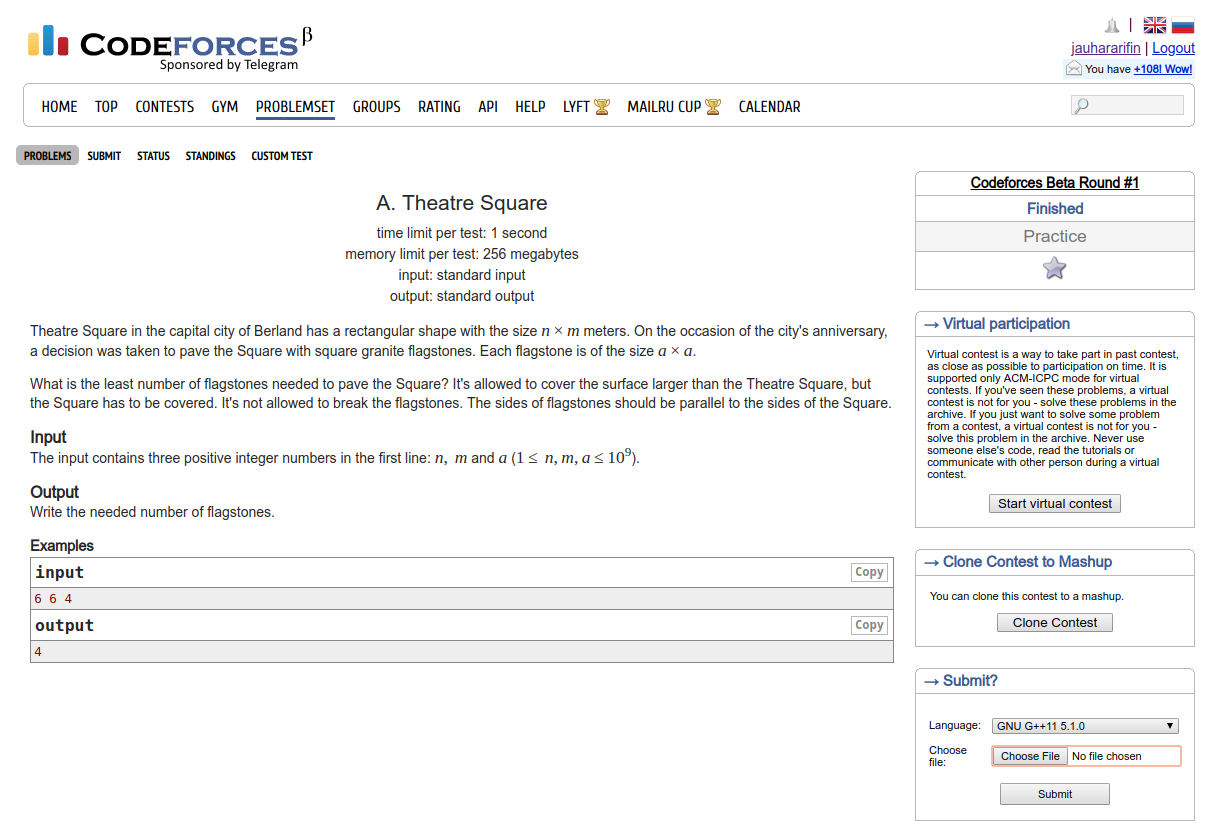
\includegraphics[width=\textwidth]{images/codeforces}
	\caption{Contoh Sistem \textit{Online Judge} : Codeforces.}
	\label{fig:codeforces}
\end{figure}

\par Beberapa organisasi memiliki \textit{online judge} yang secara publik dapat diakses, diantaranya adalah: URI \textit{Online Judge}, TOKI \textit{Online Judge}, Codeforces, Uva, SPOJ, dan lain sebagainya. \textit{Online judge} yang bersifat publik ini biasanya memiliki beberapa soal-soal yang dapat digunakan untuk latihan dan dapat dikerjakan tanpa harus berkompetisi dengan peserta lain. Pada URI \textit{Online Judge} terdapat fitur tambahan seperti forum dan \textit{rewarding system} (\cite{uriojpaper}). Terdapat beberapa sistem \textit{online judge} yang bersifat \textit{open source} seperti Mooshak, Judgels, dan DomJudge. Sistem \textit{online judge} yang bersifat open source biasanya digunakan untuk oleh beberapa instansi seperti universitas untuk membuat kompetisi \textit{competitive programming} yang bersifat privat seperti Gemastik, Compfest, Vocompfest, Arkavidia, dan INC.

\section{\textit{Autograder}}

\par \textit{Autograder} merupakan suatu aplikasi yang digunakan untuk melakukan kompilasi, eksekusi dan menilai sebuah \textit{source code} (\cite{danutamalms}). \textit{Autograder} digunakan dalam sistem \textit{online judge} untuk menilai kebenaran suatu \textit{source code}. Umumnya \textit{autograder} akan melakukan kompilasi pada \textit{source code} yang dikirimkan oleh peserta pada kompetisi \textit{competitive programming}. Hasil kompilasi dari kode peserta tersebut akan di-test dengan menggunakan \textit{test-case} rahasia yang telah dibuat oleh juri atau \textit{problem setter}. Setelah melalui pengetesan, program akan dinilai berdasarkan hasil tes tersebut. Gambar \ref{fig:grading-process} menjelaskan alur penilaian sebuah \textit{source code} yang dikirimkan peserta.

\begin{figure}
	\centering
	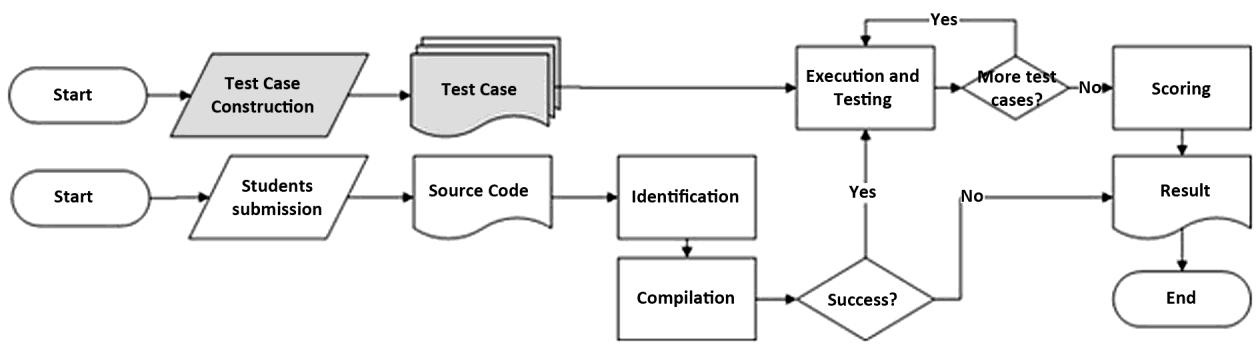
\includegraphics[width=\textwidth]{images/grading-process}
	\caption{Proses penilaian program peserta (\cite{danutamalms}}
	\label{fig:grading-process}
\end{figure}

\par Seluruh proses penilaian sebuah \textit{source code} peserta membutuhkan waktu tiga menit jika dilakukan secara manual, sedangkan hanya membutuhkan waktu sepuluh detik dengan menggunakan \textit{autograder} (\cite{danutamalms}). Dengan menggunakan \textit{autograder}, peserta kompetisi \textit{competitive programming} dapat menerima \textit{feedback} dengan lebih cepat dan mengurangi pekerjaan yang harus dilakukan oleh juri.

\par Terdapat banyak hal yang harus diperhatikan dalam membangun sistem \textit{online judge} dengan menggunakan \textit{autograder}. Salah satu permasalahan yang harus dihadapi dalam membangun \textit{autograder} adalah masalah keamanan sistem. Sistem \textit{autograder} harus dapat bertahan terhadap serangan yang mungkin dilakukan oleh peserta. Beberapa serangan yang mungkin dilakukan oleh peserta adalah mengirimkan \textit{source code} yang memiliki waktu kompilasi yang sangat lama dan membebani sistem, membuat kode yang dapat mengubah atau merusah lingkungan testing \textit{autograder}, dan mengakses \textit{resource} dari \textit{autograder} yang tidak diizinkan oleh sistem (\cite{wasikojsurvey}). Metode yang mungkin dilakukan untuk mengatasi masalah keamanan tersebut adalah dengan melakukan \textit{sandboxing}. \textit{Sandboxing} merupakan teknik mengisolasi suatu eksekusi program sehingga tidak mengganggu lingkungannya. Metode \textit{sandboxing} yang populer untuk masalah ini adalah dengan menggunakan \textit{virtualization} seperti KVM, atau menggunakan \textit{container} seperti LXC dan Docker.

\par Hal lain yang perlu diperhatikan dalam membangun \textit{autograder} adalah aspek \textit{fairness}. Waktu eksekusi program perlu diukur dengan tepat untuk menciptakan sistem yang adil. Waktu eksekusi program yang sama dengan input yang sama dapat memiliki nilai yang berbeda bergantung beberapa faktor seperti kecepatan CPU, ukuran RAM, dan lain sebagainya. Waktu pengukuran sebuah program dalam sistem \textit{autograder} biasanya dilakukan dalam hitungan milidetik. Beberapa metode yang dapat digunakan untuk mengukur waktu pemrosesan adalah dengan melakukan analisis pada \textit{hardware performance}, \textit{code instrumentation}, atau \textit{code sampling} (\cite{wasikojsurvey}). Umumnya \textit{autograder} dalam sebuah sistem \textit{online judge} memiliki banyak \textit{worker} untuk meningkatnya banyaknya program yang dapat dinilai dalam satuan waktu. \textit{Autograder} ini dapat dijalankan di komputer yang berbeda, dan dapat memiliki kinerja yang berbeda. Oleh karena itu, pengukuran waktu sangat penting dalam sistem \textit{autograder} untuk meningkatkan \textit{fairness} dari sistem.

\section{\textit{Containerization}}

\par Secara singkat \textit{container} merupakan teknologi virtualisasi program pada tingkat sistem operasi, berbeda dengan teknik virutalisasi menggunakan \textit{hypervisor} yang bekerja pada tingkat \textit{hardware} (\cite{merkeldocker}). \textit{Container} bekerja seperti \textit{virtual machine} yang dapat memberikan isolasi terhadap program yang berjalan. Pada \textit{virtual machine}, virtualisasi terjadi pada tingkat \textit{hardware} sehingga pengguna perlu menginstall sistem operasi pada lingkungan yang terisolasi untuk dapat menjalankan program. Pada \textit{container}, pengguna tidak perlu menginstall sistem operasi karena virtualisasi terjadi pada tingkat \textit{software} sehingga sistem operasi dari \textit{host} dapat digunakan dalam \textit{container}. Hal tersebut membuat \textit{container} lebih ringan dibandingkan \textit{virtual machine} karena tidak ada kerja tambahan untuk menjalankan sistem operasi baru. Gambar \ref{fig:docker-architecture} mengilustrasikan arsitektur salah satu \textit{container} yang populer yaitu Docker.

\begin{figure}
	\centering
	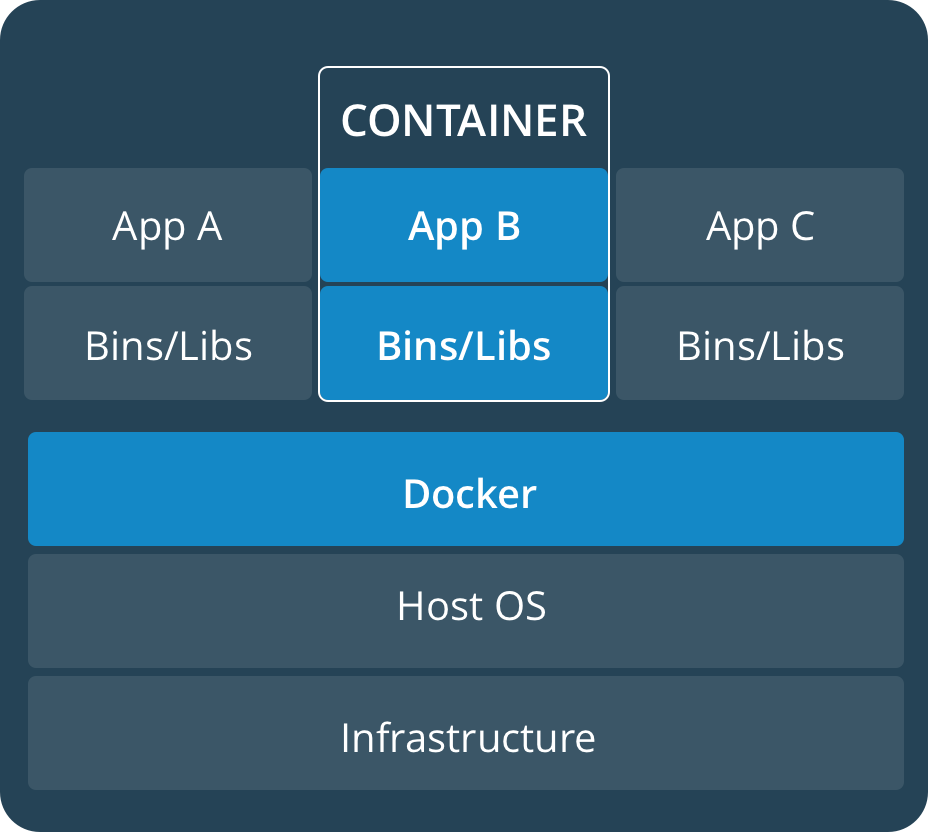
\includegraphics[width=0.5\textwidth]{images/docker-architecture}
	\caption{Arsitektur \textit{container} pada Docker (\cite{dockerdocs}).}
	\label{fig:docker-architecture}
\end{figure}

\par Pada \textit{linux}, teknologi mungkin dilakukan karena adanya beberapa fitur dari \textit{linux} yaitu: \textit{chroot}, \textit{cgroup} dan \textit{namespace}. \textit{Cgroup} dapat memberikan isolasi \textit{file system} terhadap suatu program yang berjalan pada \textit{linux}. \textit{Cgroup} dapat memberikan batasan \textit{resource} kepada suatu program yang berjalan pada \textit{linux}. \textit{Namespace} dapat memberikan isolasi pada program sehingga program dalam suatu lingkungan tidak dapat mengetahui adanya program pada lingkungan lain. Terdapat beberapa perangkat lunak yang menawarkan teknologi \textit{containerization} ini, yang populer diantaranya adalah: Docker dan LXC. Dengan menggunakan Docker atau LXC, pengguna dapat membuat suatu lingkungan yang tersiolasi untuk menjalankan suatu program tertentu tanpa mengganggu lingkungan diluar lingkungannya. Docker memberikan \textit{API} yang lebih \textit{high-level} dibandingkan dengan LXC, dan memiliki banyak fitur yang dapat digunakan untuk mengelola \textit{container}. Docker biasanya digunakan sebagai \textit{platform} untuk mendeploy aplikasi.

\par Teknologi \textit{container} dapat digunakan untuk melakukan penilaian terhadap kode program yang dikirimkan oleh peserta kompetisi \textit{competitive programming}. Dengan menggunakan \textit{container}, program yang dijalankan dapat diisolasi sehingga tidak membahayakan lingkungan. Selain itu, \textit{resource} seperti \textit{CPU usage}, \textit{memory}, \textit{storage}, dan IO pada \textit{container} dapat dibatasi sehingga tidak mengganggu program lain yang sedang berjalan pada lingkungan di luar \textit{container} (\cite{merkeldocker}).

\section{\textit{Chroot}}

\par \textit{Chroot} merupakan \textit{system call} pada sistem operasi yang berbasis \textit{linux} atau \textit{unix}. \textit{System call} ini dapat mengubah \textit{root file system} ke direktori target tertentu kemudian menjalankan program. Program yang dijalankan seakan-akan memiliki direktori \textit{root} sebagai direktori yang dispesifikasi pada waktu pemanggilan \textit{system call} \textit{chroot}. Dengan mengguakan cara ini, program yang dijalankan dalam \textit{chroot} hanya dapat mengakses \textit{file system} yang berada pada direktori target saja dan mengurangi kemungkinan serangan yang mungkin dilakukan pada \textit{file system} asli (\cite{lessardchroot}). Dengan menggunakan \textit{chroot}, pengguna dapat mengatur \textit{library} apa saja yang dapat digunakan oleh program yang berjalan dalam lingkungan \textit{chroot}. Hal ini dapat menjadi merepotkan karena pengguna perlu memasukkan semua \textit{library} yang dibutuhkan ke dalam \textit{file system} \textit{chroot}. Teknologi \textit{container} memanfaatkan \textit{chroot} untuk mengisolasi \textit{file system} yang dapat diakses oleh program yang berjalan pada \textit{container}.

\par Meskipun \textit{chroot} memberikan penghalang pada aplikasi yang berada dalam lingkungan \textit{chroot} untuk mengakses \textit{file system} yang berada di luar lingkungan direktori target, \textit{chroot} masih memiliki kelemahan. Jika aplikasi yang berjalan pada lingkungan \textit{chroot} memiliki root permission, maka aplikasi tersebut dapat dengan mudah keluar dari lingkungan \textit{chroot}. Terdapat beberapa cara untuk meningkatkan keamanan \textit{chroot} sehingga program yang berjalan di dalam \textit{chroot} sulit  untuk keluar dari lingkungan tersebut.

\par Salah satu cara untuk meningkatkan keamanan pada lingkungan \textit{chroot} adalah dengan memasukkan file yang hanya dibutuhkan oleh program saja. Sebagai contoh, jika program membutuhkan daftar user yang berada dalam sistem, di dalam linkungan \textit{chroot} perlu ada file /etc/passwd untuk mendapatkan informasi ini. Akan tetapi, file /etc/shadow tidak perlu dimasukkan ke dalam \textit{file system} \textit{chroot} karena mengandung informasi rahasia yang tidak diperlukan oleh program yang berada dalam lingkungan \textit{chroot}.

\par Cara kedua untuk meningkatkan keamanan lingkungan \textit{chroot} adalah dengan tidak memberikan akses \textit{root} kepada program yang berjalan di dalam \textit{chroot}. Terdapat beberapa serangan yang memungkinkan program dalam lingkungan \textit{chroot} untuk keluar dari lingkungan \textit{chroot} jika memiliki akses \textit{root}. Untuk menghindari jenis serangan ini, sebaiknya program yang berjalan di dalam lingkungan \textit{chroot} dibuat agar tidak mungkin mendapatkan akses \textit{root}. Tidak memberikan akses \textit{root} kepada program akan mengurangi kemungkinan adanya serangan. Akan tetapi, meskipun tidak memberikan akses \textit{root}, masih terdapat beberapa serangan yang memungkinkan program membangkitkan akses \textit{root} tanpa memiliki akses \textit{root} pada saat dijalankan.

\par Untuk meningkatkan keamanan pada lingkungan \textit{chroot}, sebaiknya tidak memasukkan \textit{hard link} ke dalam \textit{file system} \textit{chroot}. \textit{Hard link} yang mengacu pada file di luar lingkungan \textit{chroot} akan mengurangi keamanan \textit{chroot} karena memungkinkan program yang berada di dalam lingkungan \textit{chroot} untuk mengakses file yang berada di luar lingkungan \textit{chroot}.

\section{\textit{Cgroup}}

\par \textit{Cgroup} merupakan fitur pada \textit{linux} yang dapat digunakan untuk membatasi \textit{resource} yang digunakan oleh suatu kelompok program (\cite{wfeltervmcontainer}). \textit{Resource} yang dimaksud di sini adalah \textit{CPU usage}, \textit{memory usage}, \textit{disk IO} dan \textit{network IO}. Dengan menggunakan \textit{cgroup}, sebuah program yang dibatasi \textit{resource}-nya tidak akan mengganggu program lain dengan cara menghabiskan \textit{resource}. Fitur \textit{cgroup} dimanfaatkan oleh teknologi \textit{container} untuk membatasi \textit{resource} pada sebuah \textit{container} sehingga tidak membebani program lain di luar \textit{container}. Pada \textit{container}, umumnya \textit{cgroup} digunakan untuk membatasi CPU dan memori yang digunakan oleh program-program yang berjalan di dalam \textit{container}. \textit{Cgroup} dapat memberhentikan program di dalam \textit{container} jika telah menggunakan \textit{resource} yang berlebihan.

\section{\textit{Namespace}}

\par Dengan menggunakan \textit{chroot} dan \textit{cgroup}, sebuah program dapat diisolasi sehingga memiliki \textit{resource} dan \textit{file system} sendiri yang terpisah dari program-program lain yang berjalan pada \textit{host operating system}. Meskipun begitu, program yang terisolasi ini masih dapat melihat proses apa saja yang sedang berjalan pada sistem operasi karena program yang berjalan di dalam \textit{chroot} dan \textit{cgroup} masih menggunakan sistem operasi yang sama dan menggunakan kernel yang sama. \textit{Linux} memiliki fitur \textit{namespace} yang memberikan isolasi kepada program terhadap masalah ini. Dengan menggunakan \textit{namespace}, sebuah program dapat berjalan di atas \textit{namespace} tertentu dan hanya dapat mengetahui program lain yang berada di dalam \textit{namespace} yang sama. Pada \textit{container}, \textit{namespace} digunakan sehingga program yang berjalan di dalam \textit{container} hanya mengetahui program yang berada di dalam \textit{container} tersebut dan tidak dapat mengetahui program yang sedang berjalan pada \textit{host} OS-nya (\cite{wfeltervmcontainer}).

\par Selain isolasi program, \textit{namespace} juga memberikan isolasi pada hal lain seperti \textit{network}, \textit{mount}, \textit{cgroup}, \textit{user}, dan lain sebagainya. Dengan memberikan isolasi pada \textit{network}, program yang berada di dalam \textit{container} dapat membuka \textit{port} yang sama seperti program lain yang berada di \textit{container} lain. Dengan menggaunakan isolasi pada \textit{user}, \textit{user} yang ada di dalam \textit{container} tidak dapat diketahui oleh \textit{container} lain.

\section{Kernel \textit{Virtual Machine}}

\par \textit{Virtual machine} memberikan teknik virtualisasi yang berbeda dengan \textit{container}. \textit{Container} berjalan pada \textit{level} sistem operasi sedangkan \textit{virtual machine} berjalan pada \textit{level} \textit{hardware}. Pada \textit{container}, fitur-fitur dari \textit{linux} digunakan untuk mendukung virtualisasi dan isolasi program, sedangkan pada \textit{virtual machine} digunakan \textit{hypervisor} untuk melakukan virtualisasi. Dengan menggunakan \textit{virtual machine}, pengguna dapat menjalankan lebih dari satu sistem operasi berbeda di dalam komputer yang sama. Hal ini berbeda dengan \textit{container} yang hanya dapat menjalankan satu sistem operasi saja. KVM merupakan fitur dari \textit{linux} yang memungkinkan \textit{linux} menjadi \textit{hypervisor} dan menjalankan \textit{guest OS} di dalam proses \textit{linux} (\cite{wfeltervmcontainer}).

\par KVM memiliki fitur yang mirip dengan \textit{container}. Program yang berjalan di dalam \textit{virtual machine} terisolasi dari program yang ada di luar-nya. \textit{Resource} pada program yang berjalan di \textit{virtual machine} juga dapat dibatasi. Berbeda dengan \textit{container}, program yang berjalan di atas \textit{virtual machine} dikelola oleh sistem operasi yang berjalan di \textit{virtual machine} tersebut. Dengan menggunakan KVM, pengguna dapat menjalankan sistem yang benar-benar berbeda dengan \textit{linux}, tidak seperti \textit{container} yang hanya dapat menjalankan program yang berarsitektur \textit{linux}. \textit{Virtual machine} lebih berat dibandingkan \textit{container} karena untuk menjalankan program pada \textit{virtual machine} diperlukan sistem operasi sendiri yang berjalan yang mengakibatkan adanya pekerjaan tambahan untuk \textit{booting}, manajemen memori, manajemen proses, \textit{scheduling}, dan lain sebagainya.

\par KVM tidak cocok untuk digunakan dalam \textit{autograder} karena terlalu banyak pekerjaan tambahan yang diperlukan dan memberatkan sistem. Untuk mengevaluasi \textit{source code} peserta, tidak perlu menggunakan sistem operasi sendiri yang berbeda dengan sistem operasi yang menjalankan sistem \textit{autograder}. Dalam pembuatan \textit{autograder}, penggunaan teknologi \textit{container} lebih cocok untuk digunakan dibandingkan dengan penggunaan teknologi \textit{virtual machine}. \textit{Virtual machine} lebih cocok digunakan untuk melakukan pengetesan program yang membutuhkan berbagai macam sistem operasi. Selain itu \textit{virtual machine} juga kerap digunakan dalam pembuatan sistem IaaS seperti Amazon EC2, Digital Ocean Droplet dan Google Cloud Compute Engine.

\section{WebAssembly}

\par WebAssembly merupakan \textit{WebAPI} yang memungkinkan \textit{browser} untuk menjalankan \textit{low-level code} secara aman. Dulunya Javascript merupakan satu-satunya bahasa yang didukung secara \textit{native} oleh \textit{web}, akan tetapi semakin berkembangnya teknologi \textit{web} kebutuhan akan kinerja dari \textit{web} semakin tinggi. Javascript yang merupakan \textit{interpreted language} tidak dapat memberikan kinerja yang tinggi seperti bahasa-bahasa yang dikompilasi menjadi \textit{low-level code}. WebAssembly memberikan solusi yang memungkinkan \textit{browser} untuk menjalankan \textit{low-level code} pada sebuah sistem yang terisolasi dan aman. WebAssembly didesain untuk digunakan bersama-sama dengan Javascript untuk mengembangkan aplikasi \textit{web}. Sebuah aplikasi \textit{web} dapat memanfaatkan WebAssembly untuk meningkatkan kinerja dan memanfaatkan Javascript untuk fleksibilitas (\cite{mdnwebasm}).

\par Dengan menggunakan WebAssembly, \textit{browser} dapat membuat sebuah lingkungan yang terisolasi untuk menjalankan \textit{low-level code}. Lingkungan yang digunakan untuk menjalankan kode WebAssembly memiliki beberapa batasan seperti jumlah memori yang bisa digunakan, file yang bisa diakses dan lain sebagainya. Umumnya kode WebAssembly hanya dapat melakukan apa yang dapat dilakukan oleh \textit{web}. \textit{Web} tidak dapat mengakses sembarang file yang berada pada komputer, begitu juga WebAssembly. Web tidak dapat melakukan beberapa \textit{system call}, begitu juga WebAssembly. Meskipun WebAssembly dapat melakukan isolasi pada program yang berjalan, pembatasan \textit{resource} pada WebAssembly masih sulit dan tidak semudah dengan menggunakan \textit{container} ataupun \textit{virtual machine}. 

\par Kode WebAssembly berupa \textit{binary code} yang dapat dibuat dengan cara melakukan kompilasi dari beberapa bahasa seperti C, C++ dan Rust ke dalam format wasm. WebAssembly masih baru dan belum banyak bahasa pemrograman yang dapat dikompilasi menjadi WebAssembly. Bahasa pemrograman yang menggunakan \textit{interpreter} atau \textit{runtime environment} seperti Python dan Java masih sulit dijalankan di dalam WebAssembly.

\par Dalam sistem \textit{autograder}, WebAssembly tidak cocok digunakan karena berbagai alasan, yaitu: masih sedikitnya bahasa pemrograman yang dapat dikompilasi menjadi kode WebAssembly, sulitnya membatasi \textit{resource} pada WebAssembly, sulitnya melakukan perhitungan waktu, dan sulitnya menjaga keamanan. \textit{Browser} yang ada pada saati ini memiliki kemampuan untuk mengubah kode Javascript yang berjalan pada \textit{browser} tersebut, hal ini mengakibatkan munculnya celah keamanan pada WebAssembly jika digunakan untuk mengevaluasi kode peserta.

    \chapter{Analisis Masalah Dan Rancangan Solusi}

\par Dalam mengadakan kompetisi \textit{competitive programming} diperlukan sebuah sistem \textit{online judge}. Sistem \textit{online judge} memerlukan dua buah komponen utama yaitu \textit{autograder} dan sistem manajemen kompetisi. Sistem manajemen kompetisi memberikan layanan yang berhubungan dengan kompetisi seperti melihat soal, mengirim jawaban, membuat klarifikasi, dan melihat \textit{scoreboard}. Sistem \textit{autograder} berfungsi untuk melakukan penilaian terhadap jawaban yang telah dikirim secara \textit{realtime}. Gambar \ref{fig:architecture-old} menggambarkan arsitektur sistem \textit{online judge} yang saat ini sering digunakan.

\begin{figure}[ht!]
    \centering
    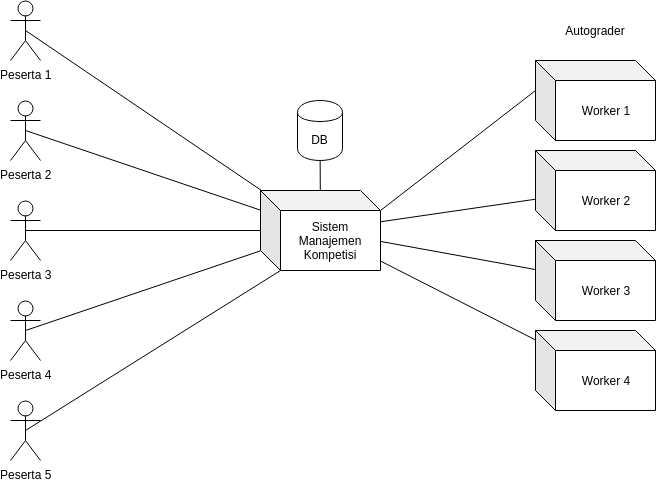
\includegraphics[width=0.7\textwidth]{images/architecture-old}
    \caption{Arsitektur Sistem \textit{Online Judge} Pada Saat Ini}
    \label{fig:architecture-old}
\end{figure}

\section{Sistem \textit{Autograder}} \label{subsec:autograder}

\par Sistem manajemen kompetisi memerlukan \textit{autograder} untuk menilai jawaban peserta kompetisi secara otomatis. Sistem \textit{online judge} yang sering digunakan saat ini menggunakan \textit{autograder} yang dipasang oleh juri pada beberapa komputer yang sudah disediakan oleh juri. Pada tugas akhir ini, diciptakan sistem \textit{autograder} yang dapat berjalan pada komputer peserta. Komputer peserta akan bertindak sebagai \textit{worker} yang menjalankan sistem \textit{autograder}. \textit{Worker} adalah komputer yang digunakan oleh sistem \textit{autograder} untuk melakukan kompilasi dan eksekusi terhadap jawaban peserta. Dalam tugas akhir ini, komputer peserta adalah \textit{worker} dari sistem \textit{autograder}. Terdapat beberapa aspek yang perlu diperhatikan dalam mengembangkan sistem \textit{autograder} seperti pengukuran waktu dan memori, \textit{load balancing}, evaluasi jawaban peserta, dan pengiriman \textit{test-case} ke \textit{worker}. Gambar \ref{fig:architecture-new} menggambarkan arsitektur sistem \textit{online judge} yang dibuat pada tugas akhir ini.

\begin{figure}[ht!]
    \centering
    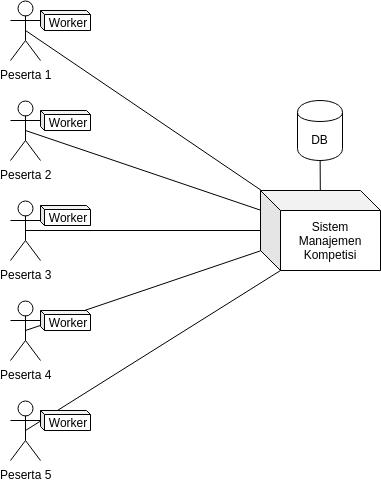
\includegraphics[width=0.5\textwidth]{images/architecture-new}
    \caption{Arsitektur Sistem \textit{Online Judge} Yang Dibuat}
    \label{fig:architecture-new}
\end{figure}

\subsection{Pengukuran Waktu Dan Memori} \label{subsec:time-memory-measure}

\par Komputer peserta memiliki spesifikasi yang berbeda-beda. Perbedaan spesifikasi tersebut menimbulkan beberapa perbedaan ketika sebuah program yang sama dieksekusi. Program yang sama dengan masukan yang sama dapat berjalan dengan waktu dan memori yang berbeda pada komputer yang berbeda. Komputer dengan \textit{clock-speed} yang lebih tinggi akan menjalankan program dengan lebih cepat. Komputer dengan \textit{core} yang lebih banyak juga akan menjalankan program parallel dengan lebih cepat. Selain itu, ukuran \textit{cache} dari komputer juga memengaruhi kecepatan waktu eksekusi. Kebutuhan memori dari suatu program juga ditentukan oleh spesifikasi komputer. Komputer dengan arsitektur 64-bit umumnya memerlukan memori yang lebih besar dibandingkan arsitektur 32-bit. Oleh karena itu, program yang dieksekusi pada komputer yang berbeda akan memerlukan waktu dan memori yang berbeda pula.

\par Penilaian jawaban peserta memerlukan metode pengukuran waktu dan memori yang adil sehingga program peserta yang benar akan dianggap benar oleh setiap \textit{worker}. Begitu juga program peserta yang salah akan dianggap salah oleh setiap \textit{worker}. Pada bab ini, dipaparkan beberapa teknik yang dapat digunakan untuk mengukur waktu eksekusi jawaban peserta.

\subsubsection{Spesifikasi CPU dan Sistem Operasi}

\par Kecepatan eksekusi sebuah program bergantung pada \textit{clock-speed} dan ukuran \textit{cache} dari CPU. Jika suatu proses hanya diberikan satu buah \textit{core} dari CPU, maka jumlah \textit{core} dari CPU dapat dianggap tidak memengaruhi kecepatan eksekusi proses tersebut. Kecepatan eksekusi program dapat diukur berdasarkan spesifikasi CPU dari komputer yang menjalankannya. Program yang dijalankan pada komputer dengan \textit{clock-speed} dan ukuran \textit{cache} yang rendah akan diberikan batasan waktu yang lebih lama. Sedangkan program yang dijalankan pada komputer dengan \textit{clock-speed} dan ukuran \textit{cache} yang lebih tinggi akan diberikan batasan waktu yang lebih singkat. Kebutuhan memori dari program yang dijalankan pada suatu komputer dipengaruhi oleh arsitektur komputer tersebut. Komputer peserta dapat memiliki arsitektur yang berbeda-beda. Komputer dengan arsitektur 64-bit umumnya memerlukan memori yang lebih besar dibandingkan dengan komputer dengan arsitektur 32-bit. Dengan mengetahui arsitektur komputer, kebutuhan memori dari suatu program dapat diperkirakan.

\par Pada penilaian jawaban peserta, diperlukan pengukuran waktu dan memori yang sangat akurat. Pengukuran waktu atau memori yang tidak akurat akan menimbulkan ketidakadilan dalam melakukan penilaian jawabab peserta. Dengan hanya memerhatikan spesifikasi dari CPU dan sistem operasi pada komputer peserta, pengukuran waktu dan memori yang akurat sulit dilakukan. Program yang berjalan pada sistem operasi 64-bit tidak selalu memerlukan memori dua kali dari program yang berjalan pada sistem operasi 32-bit. Kebutuhan memori bergantung pada isi dari program yang dijalankan dan beberapa faktor lain. Kecepatan eksekusi dari suatu program pun bergantung dari beberapa faktor lain sehingga pengukuran waktu dengan cara ini sulit untuk dilakukan.

\subsubsection{CPU \textit{Benchmarking}}

\par \textit{Benchmarking} dapat dilakukan untuk mengukur kinerja CPU dengan menggunakan sebuah program \textit{test}. Program \textit{test} dapat dijalankan pada CPU untuk mengukur waktu eksekusinya. Program \textit{test} yang dijalankan pada komputer pengguna akan dicatat jumlah instruksi dan waktunya. Jumlah instruksi dan waktu yang dibutuhkan untuk menjalankan program \textit{test} dapat digunakan untuk mengukur kinerja CPU. Batas waktu dari jawaban peserta kemudian ditentukan berdasarkan hasil eksekusi program \textit{test} tersebut.

\par \textit{Benchmarking} pada komputer peserta memiliki celah keamanan. Peserta bisa saja menjalankan program yang berat ketika proses \textit{benchmarking} dilakukan. Hal ini akan menyebabkan waktu eksekusi menjadi lambat dan dapat meningkatkan batasan waktu dari jawaban peserta.

\par Selain adanya celah keamanan, terdapat kesulitan lain yang ditemukan ketika melakukan \textit{benchmarking} yaitu pembuatan program \textit{test}. Program \textit{test} perlu dibuat sedemikian rupa sehingga dapat memberikan pengukuran waktu dan memori yang akurat. Untuk mengukur waktu eksekusi dan penggunaan memori dari program peserta dengan kompleksitas yang berbeda, diperlukan program \textit{test} yang berbeda. Hal ini mengakibatkan perlunya membuat program \textit{test} untuk setiap jenis soal yang ada pada kompetisi \textit{competitive programming}. Pembuatan program \textit{test} ini kemudian memberatkan juri karena juri perlu memikirkan program \textit{test} yang cocok sehingga dapat memberikan pengukuran waktu dan memori yang akurat.

\subsubsection{\textit{Benchmarking} Dengan Solusi Juri} \label{subsec:time-memory-measure-compare-with-jury}

\par Teknik \textit{benchmarking} sebenarnya efektif digunakan oleh \textit{autograder} untuk melakukan pengukuran waktu. Meskipun begitu, teknik \textit{benchmarking} tidak efisien dan memiliki celah keamanan jika digunakan. Juri perlu membuat sebuah program \textit{test} untuk setiap soal yang diberikan kepada peserta. Hal ini memberatkan pekerjaan juri sehingga dinilai tidak efisien. Selain itu, peserta dapat menjalankan proses yang berat pada komputernya sehingga memengaruhi keakuratan teknik \textit{benchmarking}.

\par Terdapat teknik yang dapat digunakan untuk meningkatkan efisiensi teknik \textit{benchmarking}. Teknik \textit{benchmarking} dapat menjadi lebih efisien dengan menghindari pembuatan program \textit{test} dari setiap soal pada kompetisi \textit{competitive programming}. Setiap soal dari kompetisi \textit{competitive programming} memiliki solusi yang telah dibuat juri. Solusi dari juri tersebut dapat digunakan sebagai program \textit{test}. Solusi \textit{juri} memiliki kompleksitas yang sesuai dengan soal yang telah dibuat oleh juri sehingga dapat menjadi program \textit{test} yang dapat digunakan untuk mengukur waktu eksekusi dan penggunaan memori dari program peserta secara akurat. Dengan menggunakan solusi juri sebagai program \textit{test}, juri tidak perlu membuat program \textit{test} khusus sehingga proses \textit{benchmarking} dapat menjadi lebih efisien.

\par Selain masalah efisiensi, teknik \textit{benchmarking} juga memiliki permasalahan lain yaitu bagaimana menghindari kecurangan peserta. Peserta bisa saja menjalankan proses yang berat pada komputernya sehingga mengganggu keakuratan proses \textit{benchmarking}. Hal ini menyebabkan sistem \textit{autograder} menganggap bahwa komputer peserta merupakan komputer yang lambat dan mengakibatkan jawaban peserta yang lambat bisa jadi dianggap jawaban yang benar.

\par Terdapat teknik yang dapat digunakan untuk menghindari kecurangan peserta pada paragraf sebelumnya. Pengukuran waktu yang dilakukan pada saat benchmarking dapat dilakukan dengan hanya memperhitungkan \textit{CPU Time}. \textit{CPU Time} merupakan waktu dimana proses sedang dijadwalkan untuk dieksekusi oleh \textit{CPU}. Ketika peserta menjalankan banyak proses yang berat, maka \textit{CPU} akan dijadwalkan untuk mengeksekusi proses yang terkait dengan \textit{autograder} secara lebih jarang. Hal ini dikarenakan sistem operasi membagikan \textit{CPU} secara adil untuk seluruh proses yang ada. Dengan cara ini, waktu yang dijadwalkan untuk proses lain tidak akan dihitung dalam \textit{benchmarking}.

\par Sistem operasi berbasis Linux menyediakan fitur \textit{cgroup} yang dapat digunakan untuk melakukan pengukuran \textit{CPU Time} dari suatu proses. Dengan menggunakan \textit{cgroup}, \textit{resource} yang digunakan oleh proses dapat dipantau. \textit{Cgroup} memungkinkan suatu proses untuk memantau penggunaan CPU dan memori dari proses lain. 

\begin{figure}[ht!]
    \centering
    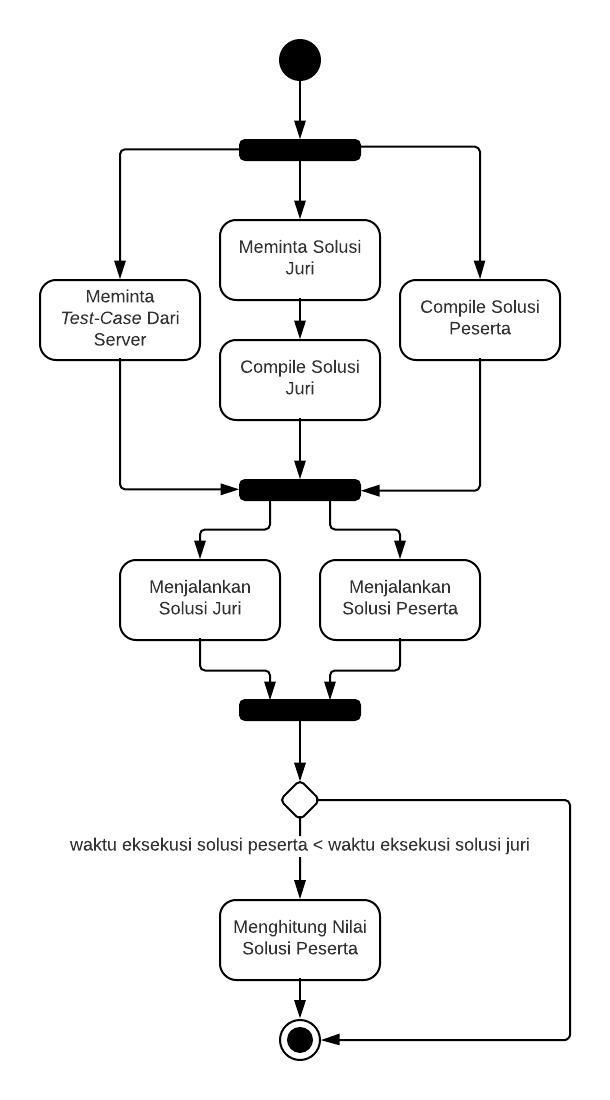
\includegraphics[width=0.5\textwidth]{images/cpu-time-counting}
    \caption{Diagram Aktivitas Penilaian Solusi Peserta}
    \label{fig:cpu-time-counting}
\end{figure}

\par \textit{Autograder} perlu menentukan apakah solusi peserta masih berada pada batas waktu yang diinginkan oleh juri. Hal tersebut dapat dicapai dengan membandingkan waktu eksekusi solusi peserta dengan waktu eksekusi solusi juri. Jika waktu eksekusi solusi peserta masih lebih cepat dari waktu eksekusi solusi juri, maka solusi peserta akan dianggap memenuhi batas waktu.

\par Meskipun solusi juri dan solusi peserta dieksekusi pada komputer yang sama. Waktu eksekusi kedua program tersebut dapat sedikit berbeda karena adanya perbedaan implementasi antara solusi peserta dan juri. Solusi peserta bisa saja lebih lambat atau lebih cepat dibandingkan dengan solusi juri. Untuk mengatasi perbedaan waktu ini, sebuah faktor toleransi dapat diterapkan pada sistem \textit{autograder}. Solusi peserta dapat diterima jika waktu eksekusinya masih berada pada batas toleransi dari solusi juri. Secara matematis, solusi peserta akan diterima jika memenuhi persamaan berikut $ T_{peserta} < (1 + \gamma) \times T_{juri}$, dengan $\gamma$ adalah nilai dari faktor toleransi.

\par Dengan membandingkan penggunaan CPU dan memori dari solusi peserta dengan solusi juri, perhitungan waktu dan memori yang akurat dapat dilakukan. Meskipun peserta menjalankan program yang berat pada saat penilaian dilakukan, perbandingan waktu eksekusi dari program solusi juri dengan program solusi peserta akan tetap sama. Oleh karena itu, teknik ini digunakan untuk melakukan pengukuran waktu dan memori dalam menyelesaikan tugas akhir ini. Gambar \ref{fig:cpu-time-counting} menjelaskan proses penilaian jawaban peserta dengan membandingkan dengan program solusi juri. 

\lstinputlisting[caption={Contoh Program yang \textit{IO bound}},label={lst:busysleeping},language=C,style=CStyle]{listings/busy-sleep.c}

\par Dengan hanya menghitung \textit{CPU Time} dari proses, terdapat masalah lain yang muncul. Peserta bisa saja mengirimkan jawaban berupa program yang bersifat \textit{IO bound}. Program yang bersifat \textit{IO bound} tidak menggunakan banyak \textit{CPU Time}. Kode \ref{lst:busysleeping} merupakan contoh program yang bersifat \textit{IO bound}. Program tersebut tidak menggunakan banyak \textit{CPU Time} karena hanya melakukan \textit{sleep}. Pada saat \textit{sleep}, proses yang berjalan tidak akan dijadwalkan untuk dieksekusi oleh \textit{CPU}. Hal tersebut menyebabkan proses dapat berjalan dengan sangat lama akan tetapi \textit{CPU Time}-nya bernilai hampir nol. Program tersebut akan mengakibatkan \textit{autograder} tidak pernah selesai melakukan pengukuran waktu karena \textit{CPU Time}-nya sangat kecil dan proses tidak pernah selesai untuk dijalankan.

\par Untuk mengatasi proses yang bersifat \textit{IO bound}, waktu eksekusi dapat dibatasi oleh \textit{wall-clock time}. \textit{Wall-clock} merupakan waktu sebenarnya dimana proses berada berada dalam sistem operasi komputer. Proses yang berjalan ketika melakukan \textit{benchmarking} dapat dibatasi \textit{Wall-clock time}-nya. Batas \textit{wall-clock time} dapat diatur sedemikian rupa sehingga dapat dipastikan bahwa solusi peserta yang melewati batas ini dipastikan tidak lolos. Salah satu contoh batas \textit{wall-clock time} adalah satu detik ditambah lamanya \textit{CPU time} dari proses eksekusi solusi juri.

\par Penentuan batas \textit{wall-clock time} sulit dilakukan pada komputer dengan spesifikasi yang berbeda-beda. Komputer yang berbeda mungkin memiliki kecepatan \textit{IO} yang berbeda. Hal ini mengakibatkan juri perlu memerhatikan spesifikasi setiap komputer peserta untuk mengatur nilai \textit{wall-clock time} yang tepat. Selain itu, setiap proses pada sistem operasi yang berbasis Linux memiliki prioritas yang dapat diatur. Peserta bisa saja menjadikan sistem \textit{autograder} memiliki prioritas rendah sehingga proses yang melakukan pengukuran waktu jarang dijadwalkan oleh sistem operasi. Hal tersebut mengakibatkan berkurangnya keakuratan proses \textit{benchmarking}.

\par Untuk mengatasi permasalahan pada paragraf di atas, kecepatan \textit{IO} dari setiap komputer peserta yang digunakan untuk pengukuran waktu dapat dibatasi sehingga seluruh komputer peserta memiliki kecepatan \textit{IO} yang sama. Selain itu, proses \textit{autograder} dapat diatur untuk memiliki prioritas yang tinggi sehingga lebih sering dijadwalkan oleh sistem operasi. Pada tugas akhir ini solusi tersebut tidak digunakan karena masih perlu adanya penelitian lebih lanjut. Pada tugas akhir ini, ketika pengukuran waktu sudah melebihi batas \textit{wall-clock time}, \textit{autograder} akan memberikan \textit{verdict} \textit{Internal Error} yang menandakan proses penilaian gagal. Penilaian yang gagal tidak akan dihitung dan akan dijadwalkan untuk dikerjakan oleh komputer peserta lain. 

\subsection{\textit{Load Balancing}}

\begin{figure}[ht!]
    \centering
    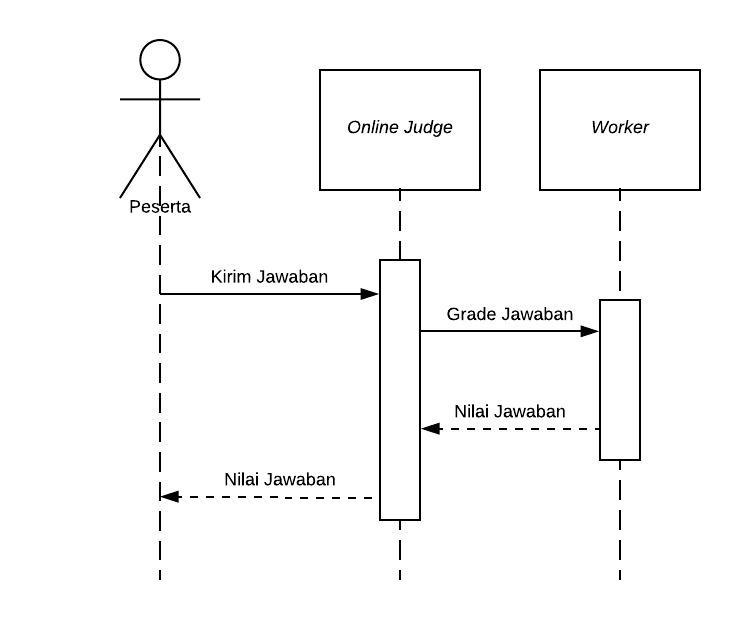
\includegraphics[width=0.75\textwidth]{images/load-balancing-push}
    \caption{\textit{Push-Based Load Balancer}}
    \label{fig:load-balancing-push}
\end{figure}

\par Dalam membangun sistem \textit{autograder}, diperlukan pembagian kerja kepada \textit{worker-worker} yang ada. \textit{Worker} yang dimaksud adalah komputer yang bekerja melakukan penilaian jawaban peserta. Dalam tugas akhir ini, \textit{worker} merupakan komputer peserta. Karena spesifikasi komputer tiap \textit{worker} berbeda-beda, diperlukan teknik pembagian kerja yang adil kepada seluruh seluruh \textit{worker}. Selain itu, aspek keamanan juga perlu diperhatikan karena jawaban peserta akan dikirimkan ke \textit{worker} lain. Terdapat beberapa pendekatan pembagian kerja yang dapat digunakan, yaitu: \textit{push-based}, \textit{pull-based}, dan \textit{self-grading}.

\par Pada pendekatan \textit{push-based}, sistem \textit{autograder} memerlukan sebuah \textit{master} yang akan membagikan pekerjaan ke seluruh \textit{worker}. \textit{Master} akan menentukan \textit{worker} mana yang akan diberikan suatu pekerjaan. Dengan menggunakan metode ini, \textit{master} perlu mengetahui informasi \textit{resource} dari seluruh \textit{worker} yang ada. Setiap \textit{worker} perlu mengirimkan informasi \textit{resource}-nya kepada \textit{master}. Metode ini cukup sulit untuk dilakukan karena perlunya mengimplementasikan algoritma \textit{load balancing} pada \textit{master}. Gambar \ref{fig:load-balancing-push} menggambarkan alur pembagian kerja dengan metode \textit{push-based}.

\begin{figure}[ht!]
    \centering
    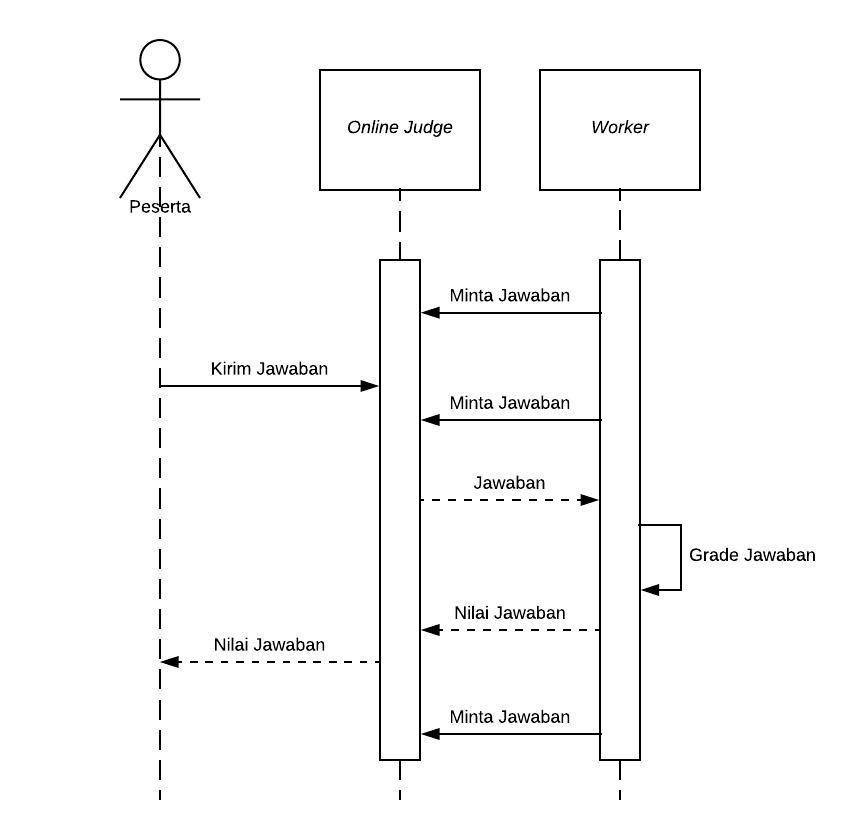
\includegraphics[width=0.75\textwidth]{images/load-balancing-pull}
    \caption{\textit{Pull-Based Load Balancer}}
    \label{fig:load-balancing-pull}
\end{figure}

\par Pada pendekatan \textit{pull-based}, diperlukan juga sebuah \textit{master} yang akan menyimpan seluruh pekerjaan yang perlu diselesaikan. Pendekatan \textit{pull-based} berbeda dengan pendekatan \textit{push-based} dimana \textit{master} lah yang memberikan pekerjaan kepada \textit{worker}. Pada pendekatan \textit{pull-based}, \textit{worker} yang sedang tersedia akan meminta pekerjaan kepada \textit{master}. Dengan pendekatan ini, pembagian pekerjaan akan menjadi rata dengan sendirinya. Metode ini lebih mudah untuk diimplementasikan dibanding dengan metode \textit{push-bashed} karena tidak perlu membuat algoritma \textit{load balancing} yang spesifik pada \textit{master}. Gambar \ref{fig:load-balancing-pull} menggambarkan alur pembagian kerja dengan metode \textit{pull-based}.

\par Selain pendekatan \textit{push-based} dan \textit{pull-based}, terdapat pendekatan lain yang lebih sederhana yaitu \textit{self-grading}. Pada \textit{self-grading}, peserta akan menilai jawabannya sendiri. Dengan menggunakan pendekatan ini, tidak diperlukan adanya \textit{master}. Meskipun begitu, pendekatan \textit{self-grading} memiliki celah keamanan karena peserta mengetahui jawaban siapa yang dinilai pada komputernya. Hal ini memungkinkan peserta untuk melakukan serangan-serangan yang mengakibatkan jawaban yang dinilai pada komputernya selalu dianggap benar.

\par Pendekatan \textit{pull-based} lebih adil dan lebih mudah diimplementasikan dibandingkan dengan pendekatan \textit{push-based}. Pendekatan \textit{pull-based} lebih aman dibandingkan dengan pendekatan \textit{self-grading} karena identitas jawaban yang dinilai pada \textit{worker} lebih rahasia. Oleh karena itu, pendekatan \textit{pull-based load balancing} digunakan pada tugas akhir ini karena lebih adil dan lebih aman dibandingkan dengan dua pendekatan lainnya.

\par Untuk meningkatkan keamanan, jawaban peserta dapat dinilai pada lebih dari satu buah \textit{worker}. Jawaban peserta dinilai benar jika mayoritas dari \textit{worker} yang menilai jawaban peserta tersebut menyatakan bahwa jawaban tersebut adalah benar. Dengan menilai jawaban peserta di banyak \textit{worker}, risiko yang timbul sebab adanya kecurangan yang dilakukan peserta dapat berkurang. Pada tugas akhir ini, \textit{load balancing} dilakukan dengan pendekatan \textit{pull-based} dan dengan melakukan penilaian jawaban peserta pada lebih dari satu buah \textit{worker}.

\subsection{Evaluasi Jawaban Menggunakan Sandbox}

\par Dalam melakukan penilaian terhadap jawaban peserta, diperlukan adanya proses kompilasi dan eksekusi terhadap program yang dikirimkan peserta. Proses kompilasi dan eksekusi ini akan dijalankan pada \textit{worker}. Proses ini dapat membahayakan lingkungan \textit{worker} jika peserta mengirimkan kode program yang berbahaya. Untuk menghindari kerusakan pada \textit{worker}, proses ini perlu diisolasi sehingga tidak berpengaruh pada lingkungan \textit{worker}. Teknik untuk mengisolasi proses eksekusi program ini dinamakan \textit{sandboxing}. Terdapat beberapa teknik \textit{sandboxing} yang dapat digunakan seperti \textit{virtual machine} dan \textit{containerization}.

\subsubsection{Menggunakan \textit{Virtual Machine}}

\par \textit{Virtual machine} memberikan isolasi kepada program pada tingkat \textit{hardware}. Komputer yang ada pada saat ini memiliki \textit{hypervisor} yang dapat digunakan untuk menyimulasikan \textit{hardware} dari komputer. Dengan menggunakan \textit{virtual machine}, komputer dapat menjalankan sistem operasi virtual di atas sistem operasi yang sedang berjalan. \textit{Virtual machine} memberikan layanan isolasi yang sangat aman.

\par Meskipun keamanan \textit{virtual machine} sangat tinggi, akan tetapi banyak \textit{overhead} yang ditimbulkan. Untuk menyalakan \textit{virtual machine}, membutuhkan waktu yang lama dan memori yang cukup besar. Selain itu, diperlukan adanya sistem operasi baru yang berjalan di atas \textit{virtual machine} yang dibuat. Hal ini menyebabkan proses penilaian jawaban peserta menjadi lambat dan membutuhkan sangat banyak memori.

\subsubsection{Menggunakan \textit{Container}}

\par \textit{Container} merupakan suatu teknik untuk mengisolasi proses pada tingkat \textit{software}. Dengan menggunakan \textit{container}, proses yang berjalan pada sistem operasi berbasis Linux dapat dibatasi \textit{resource}-nya. Penggunaan memori dan CPU dari suatu proses dapat dibatasi sehingga tidak membebani komputer peserta. Selain itu, Linux memiliki fitur yang memungkinkan pengguna mengisolasi suatu proses sehingga proses tersebut tidak dapat mengatahui informasi rahasia yang ada pada komputer peserta. \textit{Container} dapat dibuat dengan memanfaatkan fitur dari sistem operasi berbasis Linux yaitu: \textit{chroot}, \textit{namespace}, \textit{rlimit} dan \textit{cgroup}. Pada tugas akhir ini, \textit{container} digunakan untuk melakukan isolasi pada proses yang berjalan pada komputer peserta. Teknik ini dipilih karena memberikan isolasi yang cukup, dan tidak menimbulkan \textit{overhead} yang sangat besar seperti teknik isolasi dengan \textit{virtual machine}.

\par \textit{Chroot} memungkinkan proses pada sistem operasi berbasis Linux untuk memiliki \textit{filesystem} sendiri. Hal ini dapat dilakukan dengan mengganti \textit{root} dari proses ke \textit{directory} tertentu. Dengan mengganti \textit{root}, maka proses tidak dapat mengakses \textit{file} yang berada di luar \textit{directory root}. \textit{Chroot} dapat dilakukan dengan melakukan pemanggilan \textit{system call chroot}. \textit{System call chroot} hanya dapat dilakukan oleh proses yang memiliki akses \textit{root} atau memiliki \textit{capability} \textit{CAP\_SYS\_CHROOT}. Pada tugas akhir ini, program \textit{autograder} diberikan akses \textit{root} sehingga dapat melakukan pemanggilan \textit{system call chroot}.

\par \textit{Namespace} merupakan fitur dari Linux yang memungkinkan pengisolasian suatu proses sehingga tidak mengetahui informasi lain di luar \textit{namespace}-nya. Setiap proses pada Linux memiliki \textit{namespace}. Proses yang berada pada \textit{namespace} tidak akan mengetahui informasi dari \textit{namespace} lain. Hal ini memungkinkan suatu proses untuk diisolasi sehingga tidak mengatahui adanya proses lain, \textit{user} lain, ataupun \textit{network interface} lain. Dengan menggunakan \textit{namespace}, keamanan dari lingkungan \textit{worker} dapat dijaga karena jawaban peserta tidak mengetahui informasi mengenai komputer peserta. Pada tugas akhir ini, proses evaluasi jawaban peserta dilakukan di dalam \textit{namespace} yang terpisah dari \textit{namespace} pengguna.

\par Setiap proses pada sistem operasi berbasis Linux memiliki batas \textit{resource} yang dapat digunakan. Batas tersebut dapat diatur dengan melakukan pemanggilan \textit{system call setrlimit}. Proses yang menggunakan \textit{resource} melebihi batas akan dihentikan oleh sistem operasi. Pada tugas akhir ini, \textit{system call setrlimit} digunakan untuk membatasi jumlah proses yang dapat diciptakan, jumlah \textit{open file descriptor} yang dapat dimiliki, dan ukuran file yang dapat diciptakan oleh program peserta.

\par \textit{Cgroup} merupakan fitur dari sistem operasi berbasis Linux yang dapat digunakan untuk membatasi penggunaan \textit{resource} suatu proses. Selain itu, \textit{cgroup} juga dapat digunakan untuk memantau penggunaan \textit{resource} dari proses tersebut. Pada tugas akhir ini, \textit{cgroup} digunakan untuk mengukur penggunaan CPU dan memori dari proses yang berjalan dan menghentikan proses yang menggunakan \textit{resource} secara berlebihan.

\subsection{Kompilasi Program}

\par Penilaian terhadap jawaban peserta memerlukan adanya tahap kompilasi agar program dapat dijalankan. Keamanan dari proses kompilasi tentunya juga perlu dijaga. Keamanan dari proses kompilasi dapat dicapai dengan menggunakan \textit{sandbox} seperti yang sudah dijelaskan pada subbab sebelumnya.

\par Salah satu aspek yang perlu diperhatikan dalam melakukan kompilasi adalah pengadaan \textit{compiler}. \textit{Compiler} merupakan program yang digunakan untuk melakukan kompilasi kode sumber menjadi program yang dapat dijalankan pada sistem operasi. Komputer peserta tentunya perlu memiliki \textit{compiler} untuk melakukan kompilasi. Untuk menjaga keadilan, seluruh \textit{compiler} yang ada pada komputer peserta perlu memiliki versi yang sama. \textit{Compiler} dengan versi yang berbeda dapat menghasilkan program dengan kemampuan yang berbeda. Terkadang \textit{compiler} dengan versi yang lebih baru dapat memberikan optimisasi pada program sehingga berjalan dengan lebih cepat. Perbedaan versi \textit{compiler} pada komputer peserta akan memberikan ketidakadilan dalam proses penilaian.

\par Masalah pada paragraf sebelumnya diatasi dengan melengkapi \textit{autograder} dengan \textit{compiler}. Karena ukuran \textit{compiler} umumnya cukup besar, maka \textit{compiler} di-\textit{compress} ketika didistribusikan ke komputer peserta. Setiap sistem \textit{autograder} dijalankan, \textit{compiler} akan di-\textit{extract} sehingga siap digunakan.

\subsection{Pengiriman \textit{Test-Case} Ke \textit{Worker}} \label{subsec:sending-test-case-to-worker}

\par Dalam melakukan penilaian jawaban peserta perlu adanya pengiriman \textit{test-case} dari \textit{server} ke \textit{worker}. \textit{Test-case} merupakan informasi yang digunakan untuk menentukan kebenaran jawaban peserta sehingga informasi ini bersifat rahasia dan tidak boleh diketahui oleh peserta maupun orang lain di luar kompetisi. \textit{Test-case} digunakan sebagai masukan pada saat menjalankan program solusi peserta dan juri. Kebenaran dari solusi peserta dinilai dari keluaran yang dihasilkan. Salah satu cara untuk menilai kebenaran program peserta tersebut adalah dengan membandingkan keluaran program solusi peserta dengan keluaran program solusi juri. Jika keluaran solusi peserta sama seperti keluaran solusi juri, maka solusi peserta akan dianggap benar. Akan tetapi, seringkali keluaran dari program solusi peserta tidak harus sama persis dengan solusi juri. Soal pada \textit{competitive programming} seringkali memiliki lebih dari satu solusi yang sah dan tidak mungkin untuk menuliskan semua solusi satu per satu. Oleh karena itu, diperlukan juga adanya program \textit{checker} yang digunakan untuk menentukan kebenaran solusi peserta. Program \textit{checker} akan menilai kebenaran solusi peserta berdasarkan keluaran dari program solusi peserta dan program solusi juri.

\par \textit{Test-case} dan \textit{checker} merupakan informasi rahasia yang perlu dipertukarkan antara \textit{worker} dan \textit{server}. Pertukaran informasi rahasia ini dapat dilakukan dengan menggunakan teknik kriptografi dimana informasi akan dienkripsi terlebih dahulu sebelum dikirimkan. Proses enkripsi dan dekripsi dapat dilakukan pada lapisan \textit{transport} menggunakan TCP dengan TLS.

\begin{figure}[ht!]
    \centering
    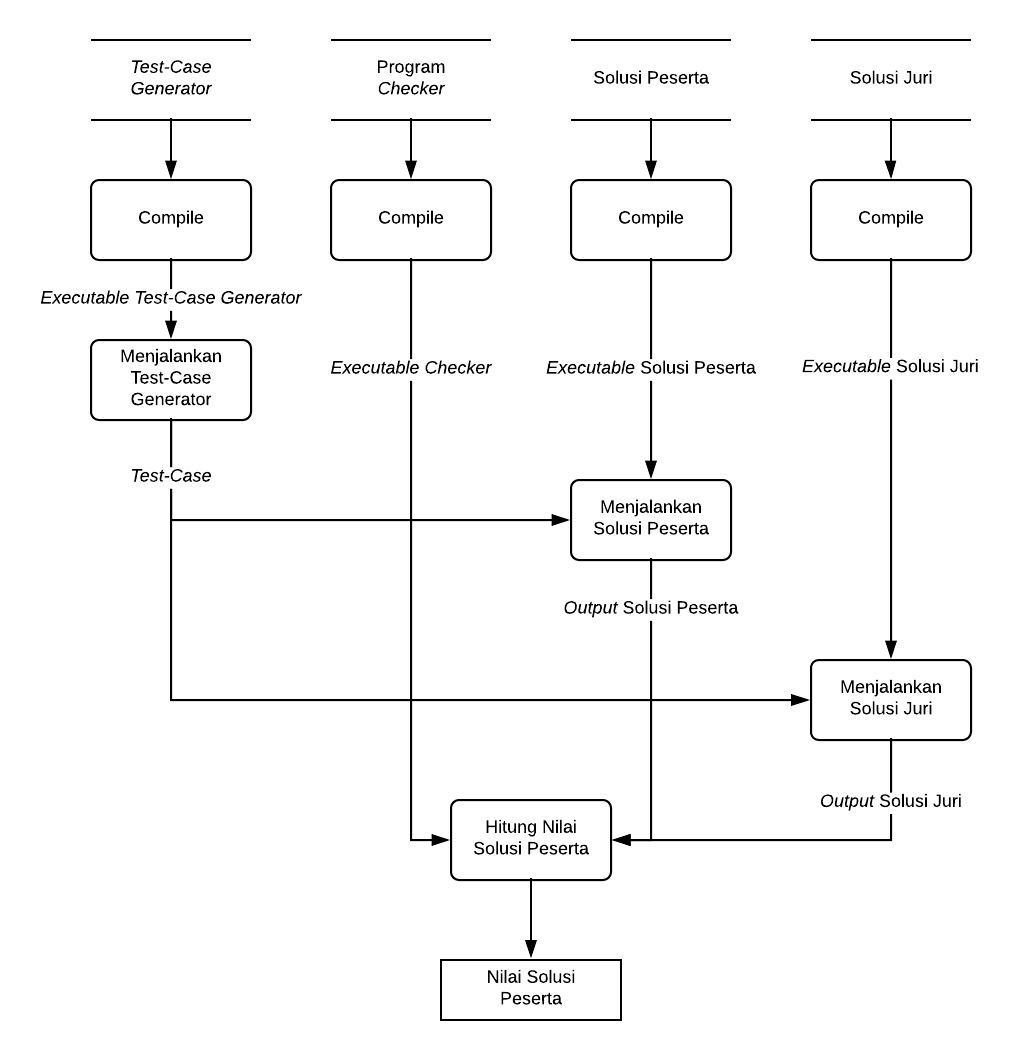
\includegraphics[width=0.85\textwidth]{images/grading-dfd}
    \caption{Diagram Aliran Data Pada Proses Penilaian Solusi Peserta}
    \label{fig:grading-dfd}
\end{figure}

\par Dengan menggunakan TCP dan TLS, kebocoran informasi yang dikirimkan melalui jaringan dapat dihindari sehingga tidak ada pihak ketiga yang dapat mengetahui isi dari informasi tersebut. Akan tetapi, karena informasi ini diterima oleh komputer peserta, peserta dapat dengan mudah mengetahui isi dari informasi tersebut. Oleh karena itu, diperlukan satu lapisan enkripsi lagi pada aplikasi yang berjalan pada komputer peserta.

\begin{figure}[ht!]
    \centering
    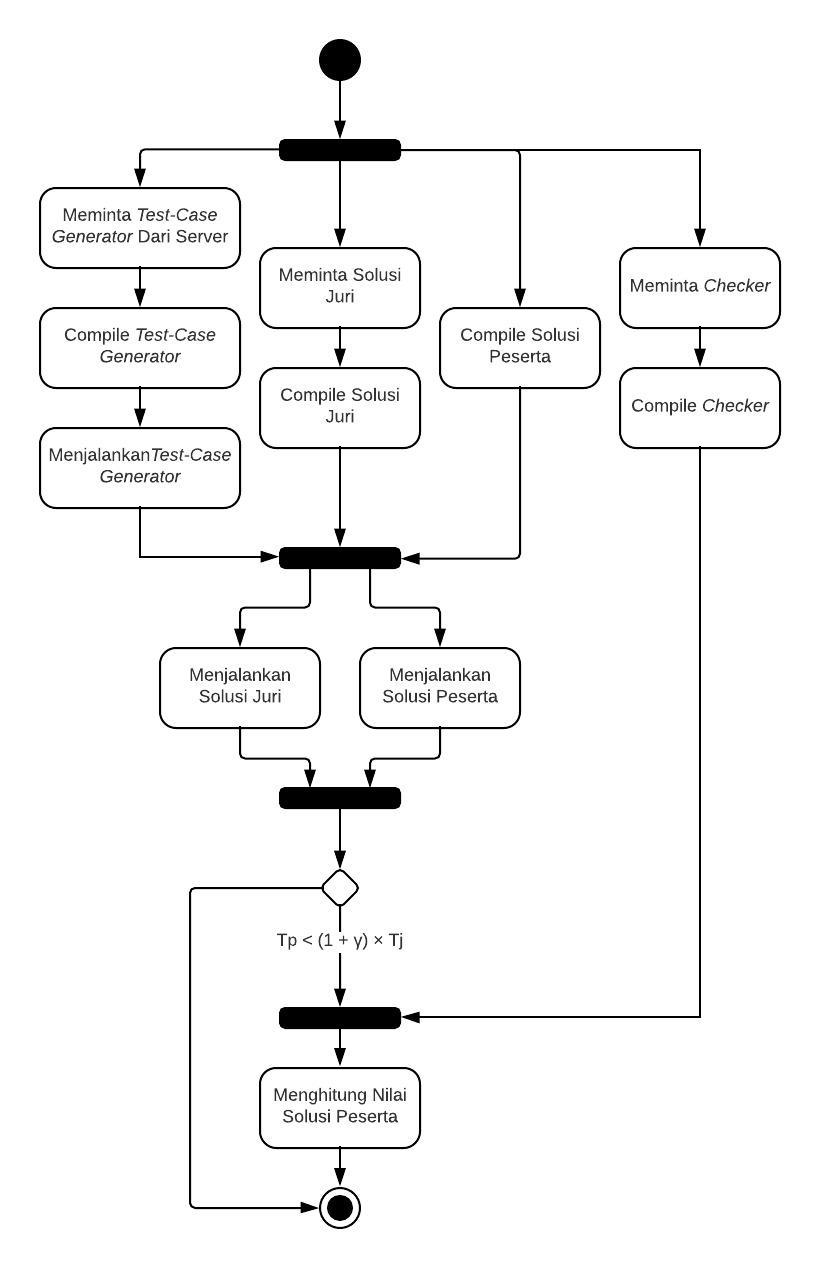
\includegraphics[width=0.65\textwidth]{images/total-grader-activity}
    \caption{Alur Proses Penilaian Jawaban Peserta}
    \label{fig:total-grader-activity}
\end{figure}

\par \textit{Test-case} umumnya merupakan file \textit{text} yang cukup besar. Pengiriman file ini dapat menghabiskan banyak \textit{bandwidth}. Meskipun begitu, \textit{test-case} biasanya dibuat dengan cara dibangkitkan oleh sebuah program yang dibuat oleh juri. \textit{Test-case} yang sama dapat dibangkitkan berulang-kali dengan menjalankan program tersebut. Untuk mengurangi kebutuhan \textit{bandwidth}, \textit{test-case} tidak perlu dikirim, melainkan program pembangkit \textit{test-case} saja yang dikirim. \textit{Test-case} yang akan digunakan untuk melakukan penilaian solusi peserta dibangkitkan dengan program pembangkit \textit{test-case} ini seperti pada Gambar \ref{fig:grading-dfd}. Diagram pada Gambar \ref{fig:total-grader-activity} menggambarkan alur proses penilaian jawaban peserta secara lengkap.

\par Pada tugas akhir ini, \textit{test-case} dipertukarkan dengan mengirimkan program pembangkit \textit{test-case} secara aman. Keamanan diperoleh dengan menggunakan dua kali enkripsi yaitu pada lapisan \textit{transport} dan aplikasi. Terdapat beberapa protokol yang dapat digunakan dalam melakukan pengiriman informasi ini. Protokol yang dipilih pada tugas akhir ini adalah protokol HTTP (\textit{hypertext transfer protocol}). Protokol ini dipilih karena aman dan mudah untuk digunakan.

\subsection{Menghadapi Serangan \textit{Reverse Engineering}}

\par Karena penilaian jawaban pada sistem \textit{online judge} yang dibangun dilakukan pada komputer peserta, maka muncul risiko adanya serangan \textit{reverse engineering} yang dapat dilakukan oleh pserta. Peserta dapat mengubah-ubah kode program dari \textit{autograder} yang dijalankan pada komputernya. Hal ini mengakibatkan peserta dapat mengubah kelakuan dari \textit{autograder}. Beberapa hal buruk yang mungkin terjadi antara lain adalah:
\begin{enumerate}
    \item Peserta dapat mengetahui kunci untuk melihat solusi juri dan \textit{testcase}.
    \item Peserta dapat selalu mengirimkan \textit{verdict} tertentu kepada sistem \textit{online judge}.
    \item Peserta dapat mengetahui jawaban dari peserta lain.
\end{enumerate}
Pada tugas akhir ini, diasumsikan peserta tidak melakukan serangan dalam bentuk \textit{reverse engineering}. Meskipun begitu, terdapat beberapa cara untuk mengurangi risiko yang muncul akibat serangan jenis ini.

\par Serangan \textit{reverse engineering} mungkin dilakukan oleh peserta jika peserta memiliki akses \textit{root} dari komputer yang digunakannya. Meskipun begitu, untuk beberapa jenis kompetisi \textit{competitive programming}, serangan ini dapat diatasi dengan tidak memberikan akses \textit{root} kepada peserta. Kompetisi ACM-ICPC merupakan salah satu jenis kompetisi yang dapat bertahan dari serangan \textit{reverse engineering}.

\par Pada kompetisi ACM-ICPC, peserta umumnya akan diseleksi terlebih dahulu secara bertingkat sebelum akhirnya berkompetisi di \textit{world final}. Sebelum babak \textit{world final}, jumlah peserta yang mengikuti kompetisi relatif sedikit sehingga sistem \textit{online judge} yang saat ini sering digunakan cukup untuk menjalankan kompetisi tersebut. Pada \textit{world final}, jumlah peserta kompetisi menjadi sangat banyak karena terdiri dari peserta-peserta yang lolos dari berbagai negara. Pada \textit{world final}, juri akan memberikan komputer khusus kepada peserta untuk mengikuti kompetisi tersebut. Pada babak \textit{world final}, juri dapat menggunakan komputer peserta sebagai \textit{worker} untuk menilai jawaban peserta. Juri dapat mengatur agar peserta tidak mendapatkan akses \textit{root} pada komputer yang digunakannya sehingga tidak dapat melakukan berbagai jenis serangan yang berupa \textit{reverse engineering}.

\par Untuk lebih mengurangi risiko yang muncul akibat serangan \textit{reverse engineering}, juri dapat mengatur agar setiap jawaban peserta dinilai oleh banyak \textit{worker}. Jika terdapat serangan \textit{reverse engineering} yang mengakibatkan \textit{worker} mengirimkan \textit{verdict} yang salah kepada \textit{server}, maka masih terdapat beberapa \textit{worker} lain yang mengirimkan \textit{verdict} yang benar. Peserta yang melakukan serangan \textit{reverse engineering} kemudian dapat dideteksi ketika \textit{verdict} yang dikirimkannya berbeda dengan peserta lain.

\par Sebagai contoh pada paragraf sebelumnya, misalkan setiap jawaban dinilai oleh lima buah \textit{worker}. Ketika sebuah jawaban dinilai, maka terdapat lima peserta berbeda yang melakukan penilain. Seorang peserta bisa saja melakukan serangan \textit{reverse engineering} dan mengakibatkan \textit{worker} pada komputernya mengirimkan \textit{verdict} yang salah kepada \textit{server}. Meskipun begitu, empat peserta lain yang tidak melakukan serangan \textit{reverse engineering} akan mengirimkan \textit{verdict} yang berbeda dengan peserta yang melakukan serangan \textit{reverse engineering}. Dengan mengamati kelima buah \textit{verdict} ini, peserta yang mengirimkan \textit{verdict} yang berbeda dapat dikatakan melakukan serangan.

% TODO: tambah cara penilaian, pikirin lagi tentang self-grading, tambah penjelasan satu jawaban bisa dinilai lebih dari satu kali, jelasin grading_size

\section{Sistem Manajemen Kompetisi}

\begin{figure}[ht!]
    \centering
    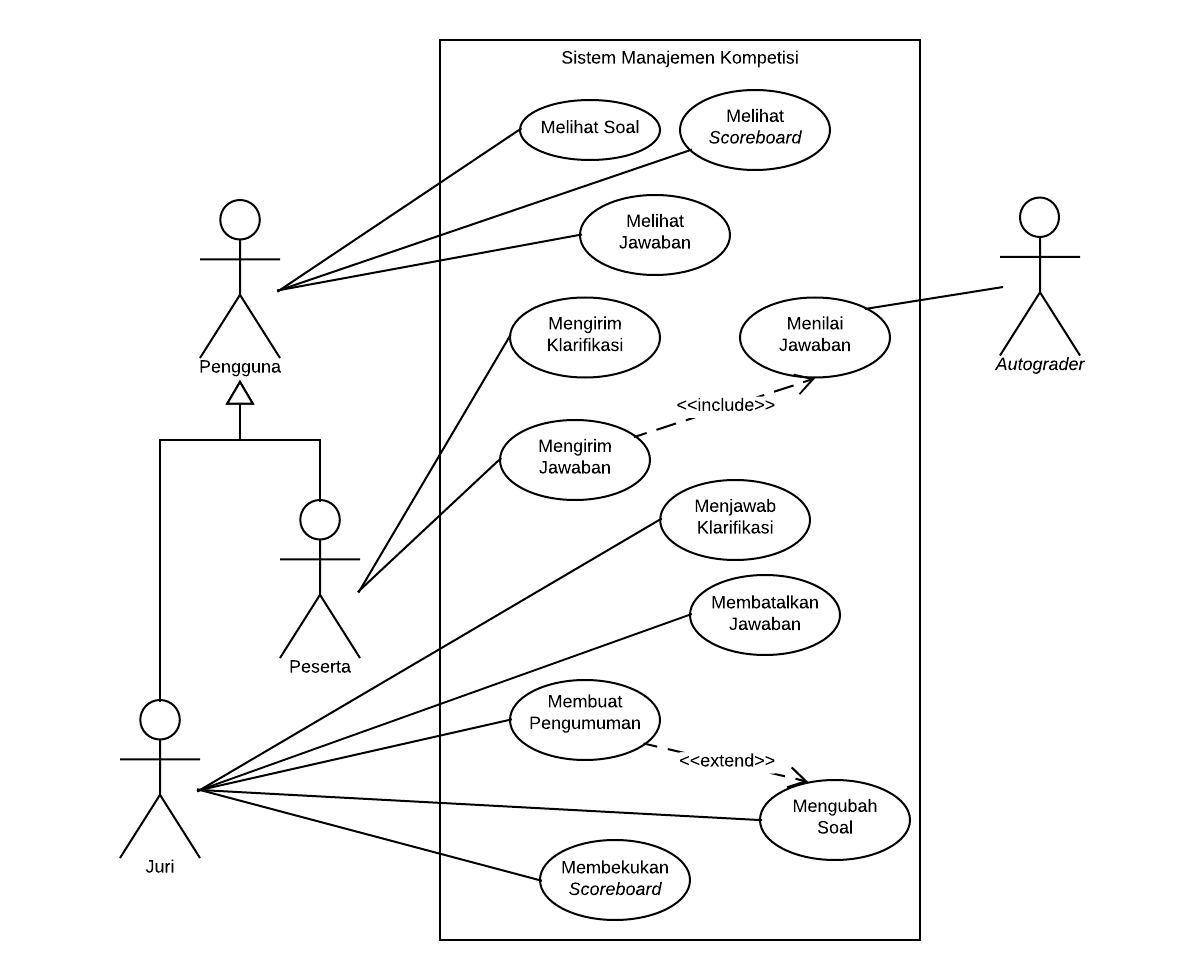
\includegraphics[width=0.85\textwidth]{images/oj-use-case}
    \caption{Diagram \textit{Use Case} Dari Sistem Manajemen Kompetisi}
    \label{fig:oj-use-case}
\end{figure}

\par Sistem manajemen kompetisi memberikan layanan kepada peserta kompetisi dan juri untuk berinteraksi. \textit{Online judge} yang populer pada saat ini memberikan sistem manajemen kompetisi berbasis \textit{web}. Sistem manajemen kompetisi ini dibutuhkan oleh peserta dan juri untuk melakukan aksi-aksi terkait kompetisi yang sedang berlangsung. Kebutuhan dari sistem manajemen kompetisi digambarkan oleh diagram \textit{use case} pada Gambar \ref{fig:oj-use-case}. Berikut ini adalah kebutuhan dari sistem manajemen kompetisi pada \textit{online judge}:

\begin{enumerate}
    \item Peserta dan juri dapat melihat soal.
    \item Peserta dapat mengirim jawaban.
    \item Sistem \textit{autograder} dapat menilai jawaban peserta.
    \item Peserta dapat mengirim klarifikasi soal.
    \item Juri dapat membuat pengumuman terkait kompetisi.
    \item Juri dapat menjawab klarifikasi peserta.
    \item Juri dapat mengubah soal.
    \item Peserta dan juri dapat melihat \textit{scoreboard}.
    \item Juri dapat membekukan \textit{scoreboard}.
    \item Peserta dapat melihat jawaban yang dikirim olehnya.
    \item Juri dapat melihat jawaban yang dikirim seluruh peserta.
    \item Juri dapat mengatur jawaban peserta untuk tidak dinilai.
\end{enumerate}

\par Pada tugas akhir ini, tidak semua kebutuhan dari sistem manajemen kompetisi diimplementasikan. Masalah yang ingin diselesaikan dalam tugas akhir ini tidak terletak pada sistem manajemen kompetisi, melainkan pada sistem \textit{autograder}. Oleh karena itu hanya kebutuhan yang berkaitan dengan proses penilaian saja yang diimplementasikan pada tugas akhir ini. Kebutuhan sistem manajemen kompetisi yang diimplementasikan pada tugas akhir ini antara lain adalah:

\begin{enumerate}
    \item Peserta dan juri dapat melihat soal.
    \item Peserta dapat mengirim jawaban.
    \item Sistem \textit{autograder} dapat menilai jawaban peserta.
    \item Juri dapat mengubah soal.
    \item Peserta dapat melihat jawaban yang dikirim olehnya.
    \item Juri dapat melihat jawaban yang dikirim seluruh peserta.
\end{enumerate}

\begin{figure}[ht!]
    \centering
    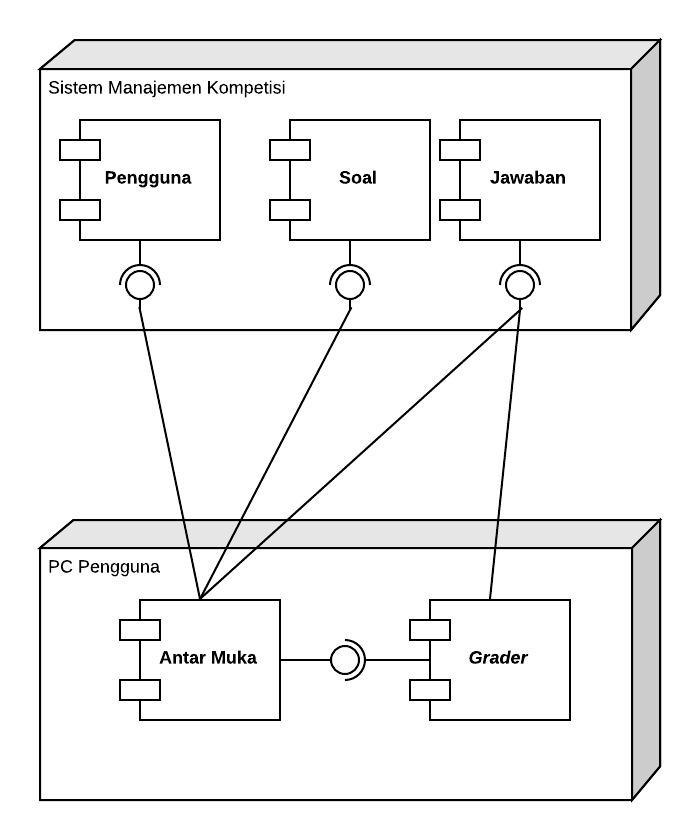
\includegraphics[width=0.5\textwidth]{images/oj-components}
    \caption{Diagram Komponen Sistem Manajemen Kompetisi}
    \label{fig:oj-components}
\end{figure}
% TODO: tambah komponen "kontes"

\par Sistem manajemen kompetisi yang digunakan pada tugas akhir ini mengikuti sistem manajemen kompetisi yang saat ini banyak digunakan. Sistem manajemen kompetisi ini dapat dibagi menjadi beberapa komponen utama yaitu: pengguna, soal, jawaban, antar muka dan \textit{grader}. Komponen \textit{grader} tidak lain adalah sistem \textit{autograder} yang telah dipaparkan pada bagian \ref{subsec:autograder}. Diagram komponen pada Gambar \ref{fig:oj-components} menggambarkan komponen yang digunakan dalam sistem manajemen kompetisi beserta keterhubungannya.

\subsection{Komponen Pengguna}

\par Kompetisi \textit{competitive programming} ada yang bersifat tertutup dimana hanya peserta tertentu yang dapat mengikutinya dan terbuka dimana setiap orang dapat mengikutinya. Sistem \textit{online judge} yang populer saat ini umumnya dapat menangani kedua jenis kompetisi tersebut. Untuk memasuki kompetisi, peserta perlu membuat akun di sistem \textit{online judge} tersebut terlebih dahulu. Peserta kemudian dapat memasuki kompetisi dengan cara melakukan \textit{login} pada sistem tersebut. Untuk menangani pendaftaran peserta baru dan \textit{login}, sistem \textit{online judge} perlu memiliki komponen manajemen pengguna yang bertugas melakukan otentikasi dan otorisasi pengguna. Beberapa \textit{online judge} memiliki komponen manajemen pengguna yang memanfaatkan layanan otentikasi dan otorisasi dari pihak ketiga seperti Google, Facebook, Github, dan Auth0. Terdapat juga sistem \textit{online judge} yang melakukan otentikasi dan otorisasi tanpa menggunakan pihak ketiga, misalnya DomJudge dan Mooshak.

\par Komponen pengguna dibuat pada sistem manajemen kompetisi untuk melakukan otentikasi dan otorisasi pengguna. Untuk menyederhanakan persoalan, pada tugas akhir ini komponen pengguna yang bertugas melakukan otentikasi dan otorisasi pengguna tidak akan menggunakan layanan pihak ketiga. Beberapa \textit{software development framework} seperti Django, Express, dan Laravel memiliki kemampuan untuk menangani masalah ini dengan mudah. Informasi pengguna akan disimpan pada sistem basis data yang sudah tersedia. Otentikasi pengguna akan dilakukan dengan sederhana, yaitu menggunakan \textit{username} dan \textit{password}.

\par Otorisasi pengguna juga dilakukan secara sederhana yaitu dengan sistem \textit{Role-based access control}. Setiap pengguna akan diberikan \textit{role} tertentu. Aksi-aksi yang dapat dilakukan oleh pengguna ditentukan oleh \textit{role} yang dimilikinya. Setiap pengguna yang berhasil \textit{login} kedalam sistem akan diberikan \textit{token} unik. \textit{Token} unik ini digunakan untuk menentukan \textit{role} dari pengguna yang melakukan aksi pada sistem. \textit{Token} yang akan digunakan dalam tugas akhir ini adalah JWT (JSON \textit{Web Token}) karena mudah untuk digunakan dan aman.

\subsection{Komponen Soal}

\par Pada kompetisi \textit{competitive programming}, deskripsi soal dapat diakses melalui sistem \textit{online judge} yang biasanya berupa halaman web. Dalam beberapa kompetisi, peserta kompetisi akan mendapatkan soal dalam bentuk \textit{hard-copy}. Komponen soal dibutuhkan oleh sistem manajemen kompetisi untuk mengelola soal yang ada pada kompetisi. Komponen ini memberikan layanan kepada pengguna untuk melihat soal. Terkadang terdapat kesalahan pada soal ketika kompetisi berlangsung sehingga komponen ini perlu memberikan layanan kepada juri untuk mengganti soal.

\par Soal pada kompetisi \textit{competitive programming} memiliki deskripsi yang merupakan penjelasan terhadap masalah yang harus diselesaikan peserta. Pada deskripsi soal terdapat penjelasan mengenai permasalahan yang dimaksud, format masukan, format keluaran, contoh masukan, dan contoh keluaran. \textit{Online judge} yang populer saat ini memberikan deskripsi soal kepada peserta dengan format \textit{pdf} atau menampilkannya dalam halaman web. Komponen soal perlu menyimpan deskripsi soal untuk dapat memberikannya kepada pengguna. Deskripsi soal dapat disimpan pada \textit{filesystem} dalam bentuk pdf atau disimpan dalam sistem manajemen basis data dalam bentuk HTML. Untuk memudahkan implementasi pada tugas akhir ini, deskripsi soal akan disimpan dalam basis data.

\par Setiap soal perlu memiliki program \textit{test-case generator}, \textit{solution}, dan \textit{checker}. Ketiga buah program ini dibuat oleh juri untuk melakukan penilaian jawaban peserta. \textit{Test-case generator} adalah program yang dibuat oleh juri untuk membangkitkan \textit{test-case} seperti yang sudah dijelaskan pada bagian \ref{subsec:sending-test-case-to-worker}. \textit{Solution} adalah program yang merupakan solusi valid dari soal. Program solusi ini dibuat oleh juri untuk dibandingkan dengan jawaban peserta seperti yang sudah dijelaskan pada bagian \ref{subsec:time-memory-measure-compare-with-jury}. Program \textit{checker} akan digunakan oleh \textit{worker} untuk menentukan kebenaran jawaban peserta. Terkadang terdapat lebih dari satu jawab yang benar pada sebuah soal. Oleh karena itu, program \textit{checker} ini dibutuhkan untuk menilai jawaban peserta. 

\par Program \textit{test-case generator}, \textit{solution}, dan \textit{checker} dapat disimpan dalam \textit{filesystem} atau sistem basis data. Pada tugas akhir ini, program-program tersebut disimpan pada \textit{filesystem} dan alamat dari program tersebut disimpan dalam sistem basis data.

\subsection{Komponen Jawaban}

\par Sistem manajemen kompetisi perlu menyediakan layanan kepada peserta untuk mengirimkan jawaban. Jawaban yang dikirimkan peserta berupa program dalam bentuk \textit{source code} dalam bahasa pemrograman yang diizinkan oleh juri. Selain itu, sistem manajemen kompetisi juga harus memberikan layanan kepada peserta untuk dapat melihat kembali jawabannya. Juri juga perlu mengawasi jawaban dari peserta untuk menghindari adanya kecurangan.  Oleh karena itu, sistem manajemen kompetisi juga harus dapat memberikan layanan kepada juri untuk melihat seluruh jawaban yang pernah dikirimkan oleh peserta. Pada sistem \textit{online judge} yang dibangun, komponen jawaban berguna untuk memberikan layanan-layanan tersebut. Pada tugas akhir ini jawaban peserta akan disimpan dalam bentuk \textit{file source code} pada \textit{filesystem}.

\subsection{Komponen Antar Muka}

\begin{figure}[ht!]
    \centering
    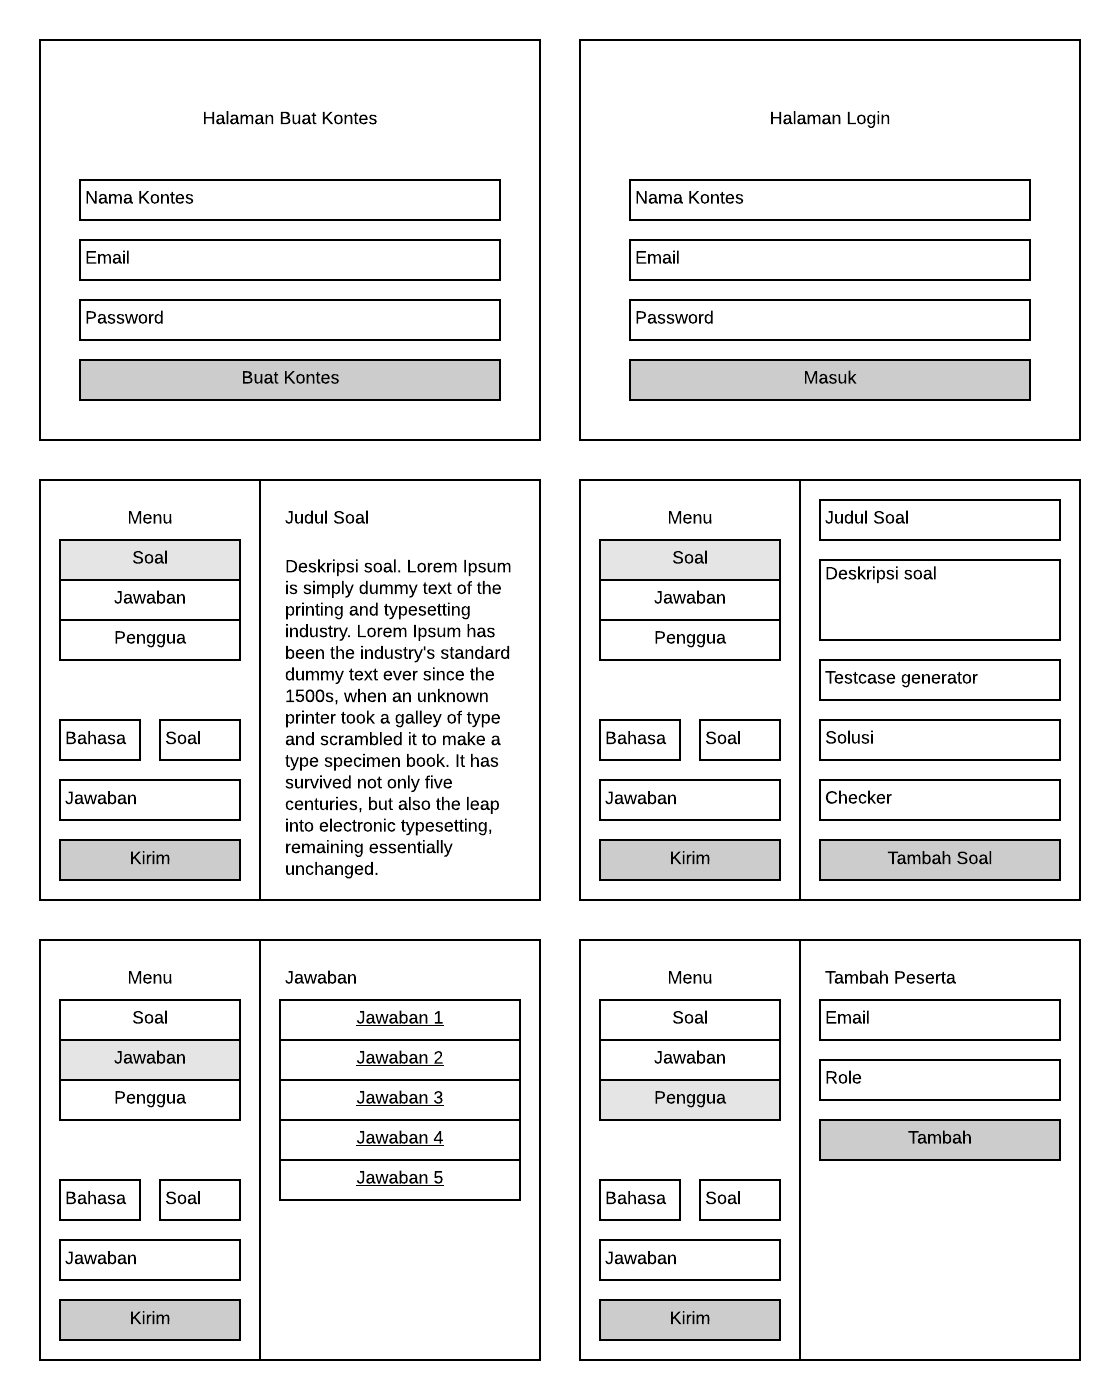
\includegraphics[width=0.85\textwidth]{images/mockup}
    \caption{Desain Tampilan Antar Muka Sistem \textit{Online Judge}.}
    \label{fig:mockup}
\end{figure}

\par Untuk memudahkan peserta dan juri berinteraksi dengan sistem \textit{online judge}, diperlukan komponen antar muka. Pengguna yang merupakan peserta dan juri menggunakan antar muka ini untuk melakukan aksi-aksi pada sistem \textit{online judge}. Kebanyakan sistem \textit{online judge} yang populer saat ini menggunakan antar muka berbasis \textit{web}. Antar muka berbasis \textit{web} digunakan karena mudah diakses oleh pengguna, dan cukup ringan untuk dijalankan.

\par Pada tugas akhir ini, antar muka dibuat dalam bentuk tampilan grafis berbasis web. Untuk memudahkan pengguna, antar muka dibuat sebagai aplikasi \textit{desktop}. Hal ini bertujuan agar komponen antar muka dan \textit{grader} dapat berjalan secara sekaligus. Gambar \ref{fig:mockup} merupakan rancangan halaman-halaman yang dibangun pada komponen antar muka.

% TODO: tambah penjelasan tentang submission, grading_group, grading, erd diagram dari db

    \renewcommand\bibname{Daftar Pustaka}
    \printbibliography

\end{document}
